\documentclass[titlepage]{article}
\usepackage{amsmath, amssymb, amsthm}
\usepackage[dvipsnames]{xcolor}
\makeatletter
\title{HolPy Integral Interface Tutorial}
\definecolor{mygray}{gray}{0.95}
\usepackage{graphicx}
\newcommand*{\rom}[1]{\expandafter\@slowromancap\romannumeral #1@}
\begin{document}
\maketitle
\tableofcontents
\section{Introduction}
HolPy integral module provides user a graphical interface to compute integrals interactively. In this tutorial, we will introduce how to use it. The interface consists of opening integral file, perform integration rules and other necessary operations when users compute an integral. In section 2, we will describe the environment requirements. In section 3, we will introduce the layout of the interface. The basic facilities and the way to apply interagtion rules on a processing integral will be introduced in Section 4.
\section{Environment}
To open the interface, the user need to install Node.js and Python3 at least. \\
After installing python and npm, switch to HolPy root directory.\\
Required python packages are listed in requirements.txt. To install required packages, use (\textcolor{red}{depending on your system, may need to replace python by python3 or python3.x)}:\\
\centerline{\colorbox{mygray}{\small{python -m pip install -r requirements.txt}}}\\
The user interface is built using Vue, in the ./app folder. To start, change to ./app and use \colorbox{mygray}{npm install} followed by \colorbox{mygray}{npm run serve}, then start the server (in the root directory) using \colorbox{mygray}{python app.py}, and go to page \colorbox{mygray}{localhost:8080}. You are successful if can see the page like this:\\

\includegraphics[bb=0 0 300 200]{1.png}\\
\section{Layout}
User can see the main page after clicking the `integral` in \colorbox{mygray}{localhost:8080}.\\
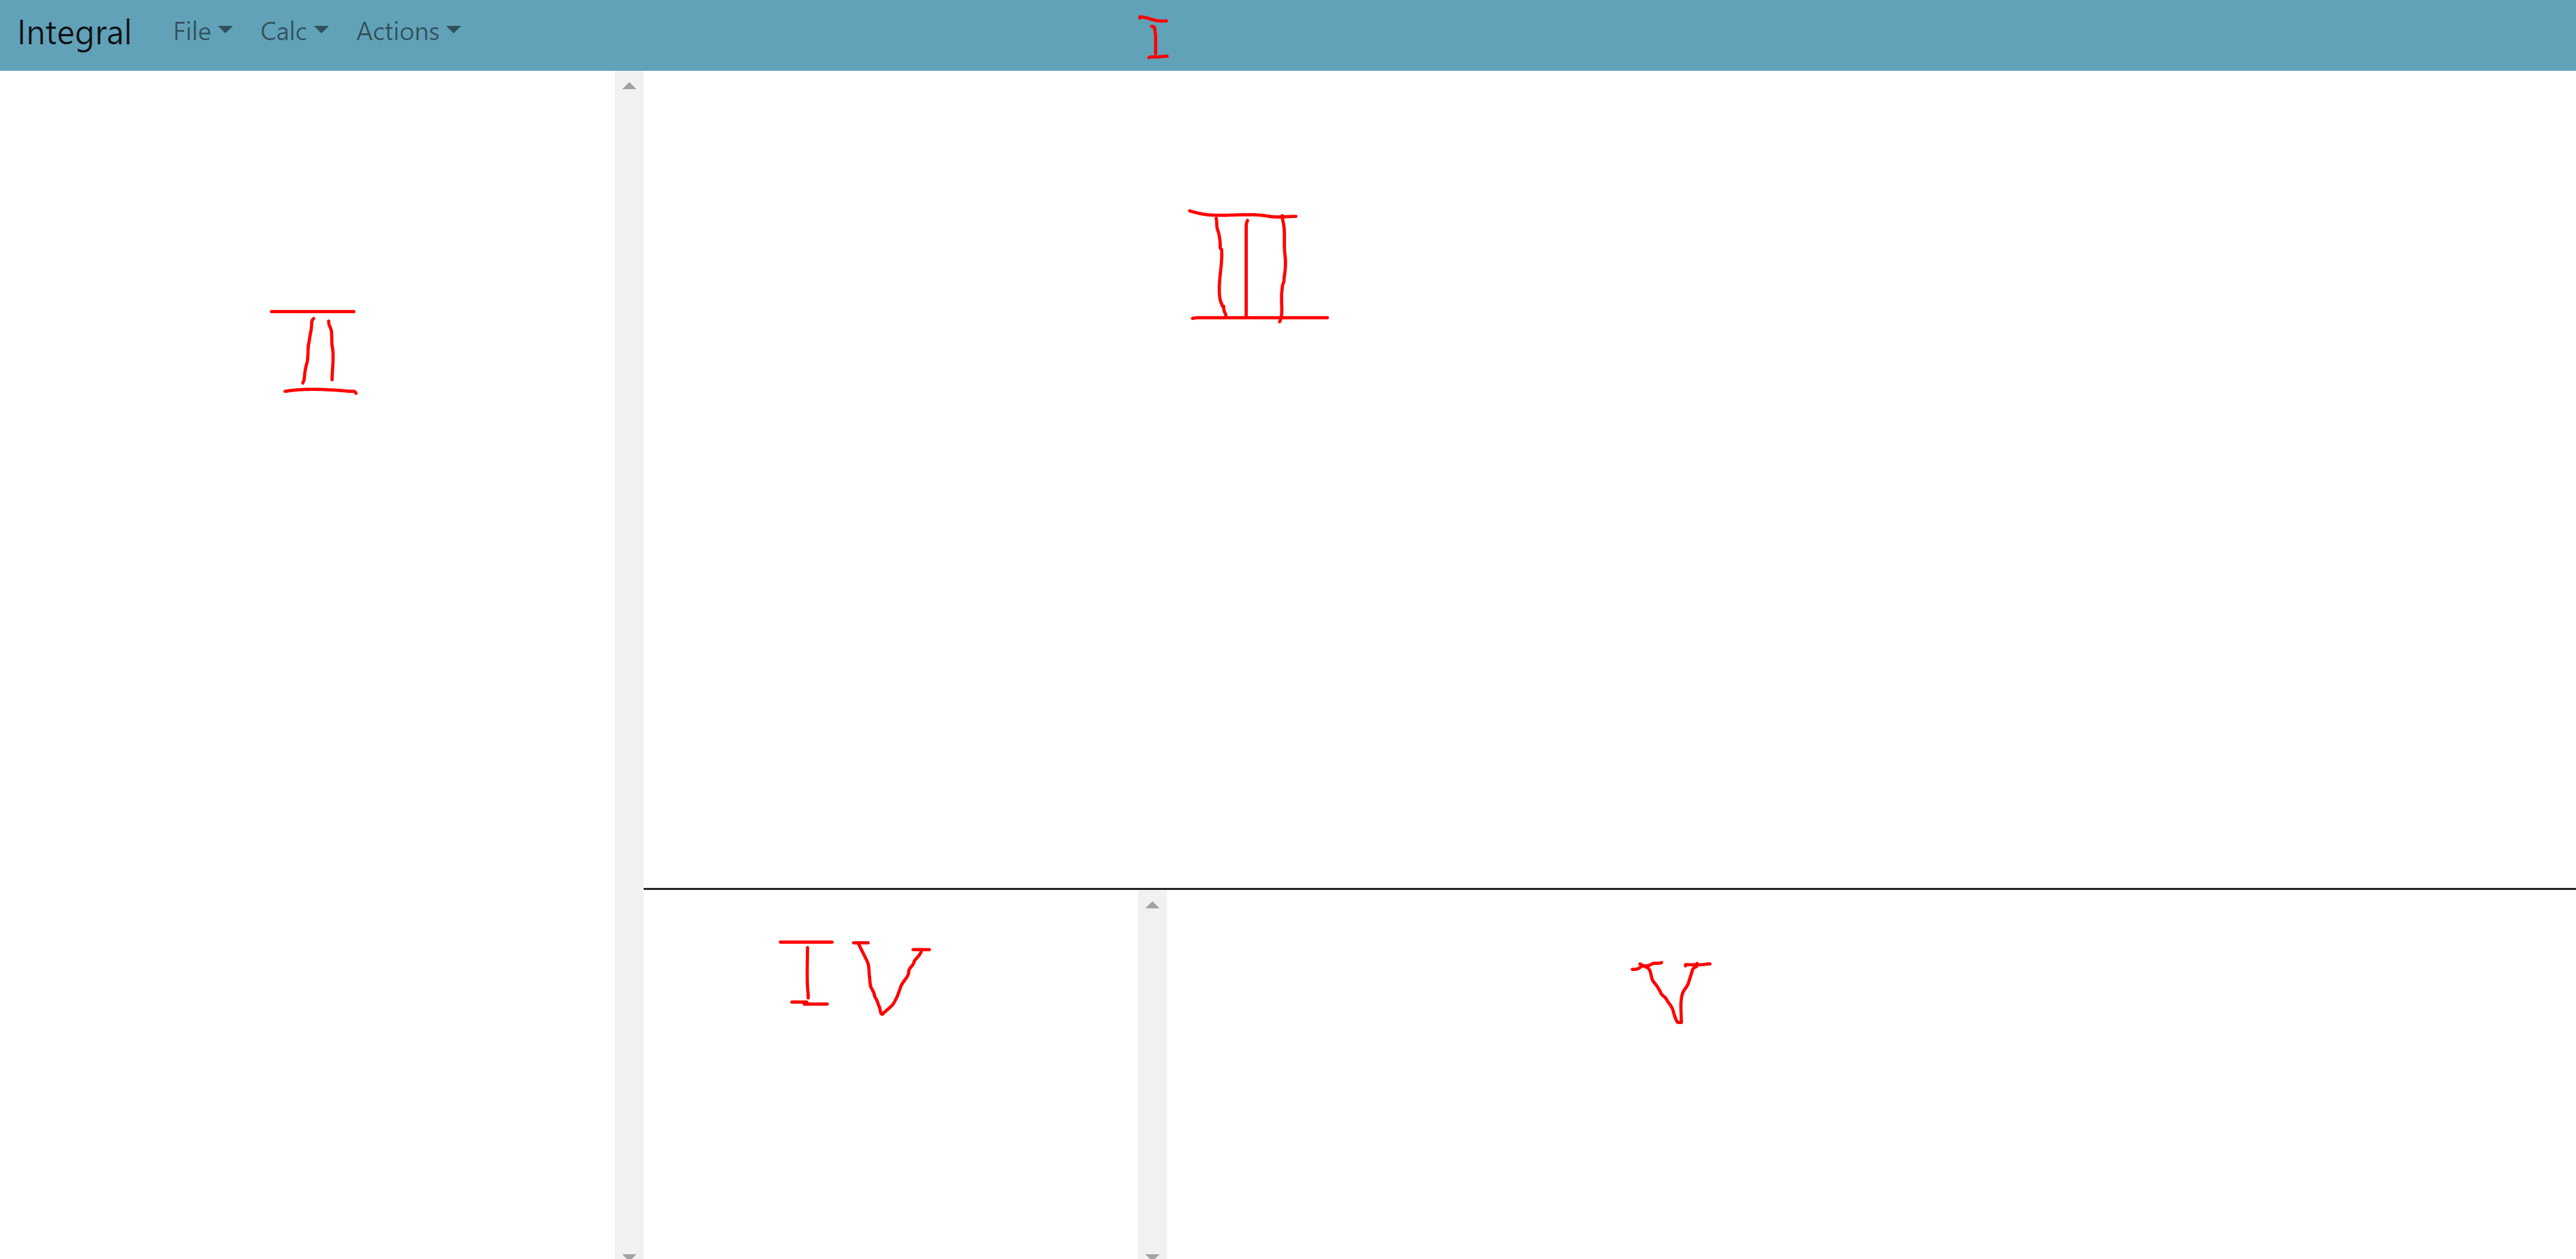
\includegraphics[width=13cm, height=7cm]{2.png}\\
For convenience, the layout is separated into 5 parts as above.\\
\rom{1}: Place operations, including open integral file, apply integration rules and so on.\\
\rom{2}: Display all the integrals existed in the opened integral file, user can click each integral and solve it.\\
\rom{3}: Display the current procedure during solving the selected integral.\\
\rom{4}: Display the integrals existed in the current solving step and user can choose one of them to apply an integration rule on it.\\
\rom{5}: User will write necessary information in this part when apply an integration rule. \\
In the following, we will use the Roman numerals to represent each part.
\section{Basic operations}
\subsection{Open file}
In the integral module, all integrals and their solutions are stored in a json file which are stored in the ./integral/example directory. User need to click the \colorbox{mygray}{Open} button in File menu to open them. For example, the following figure shows how to open examples in ./integral/example/tongji7.json:\\
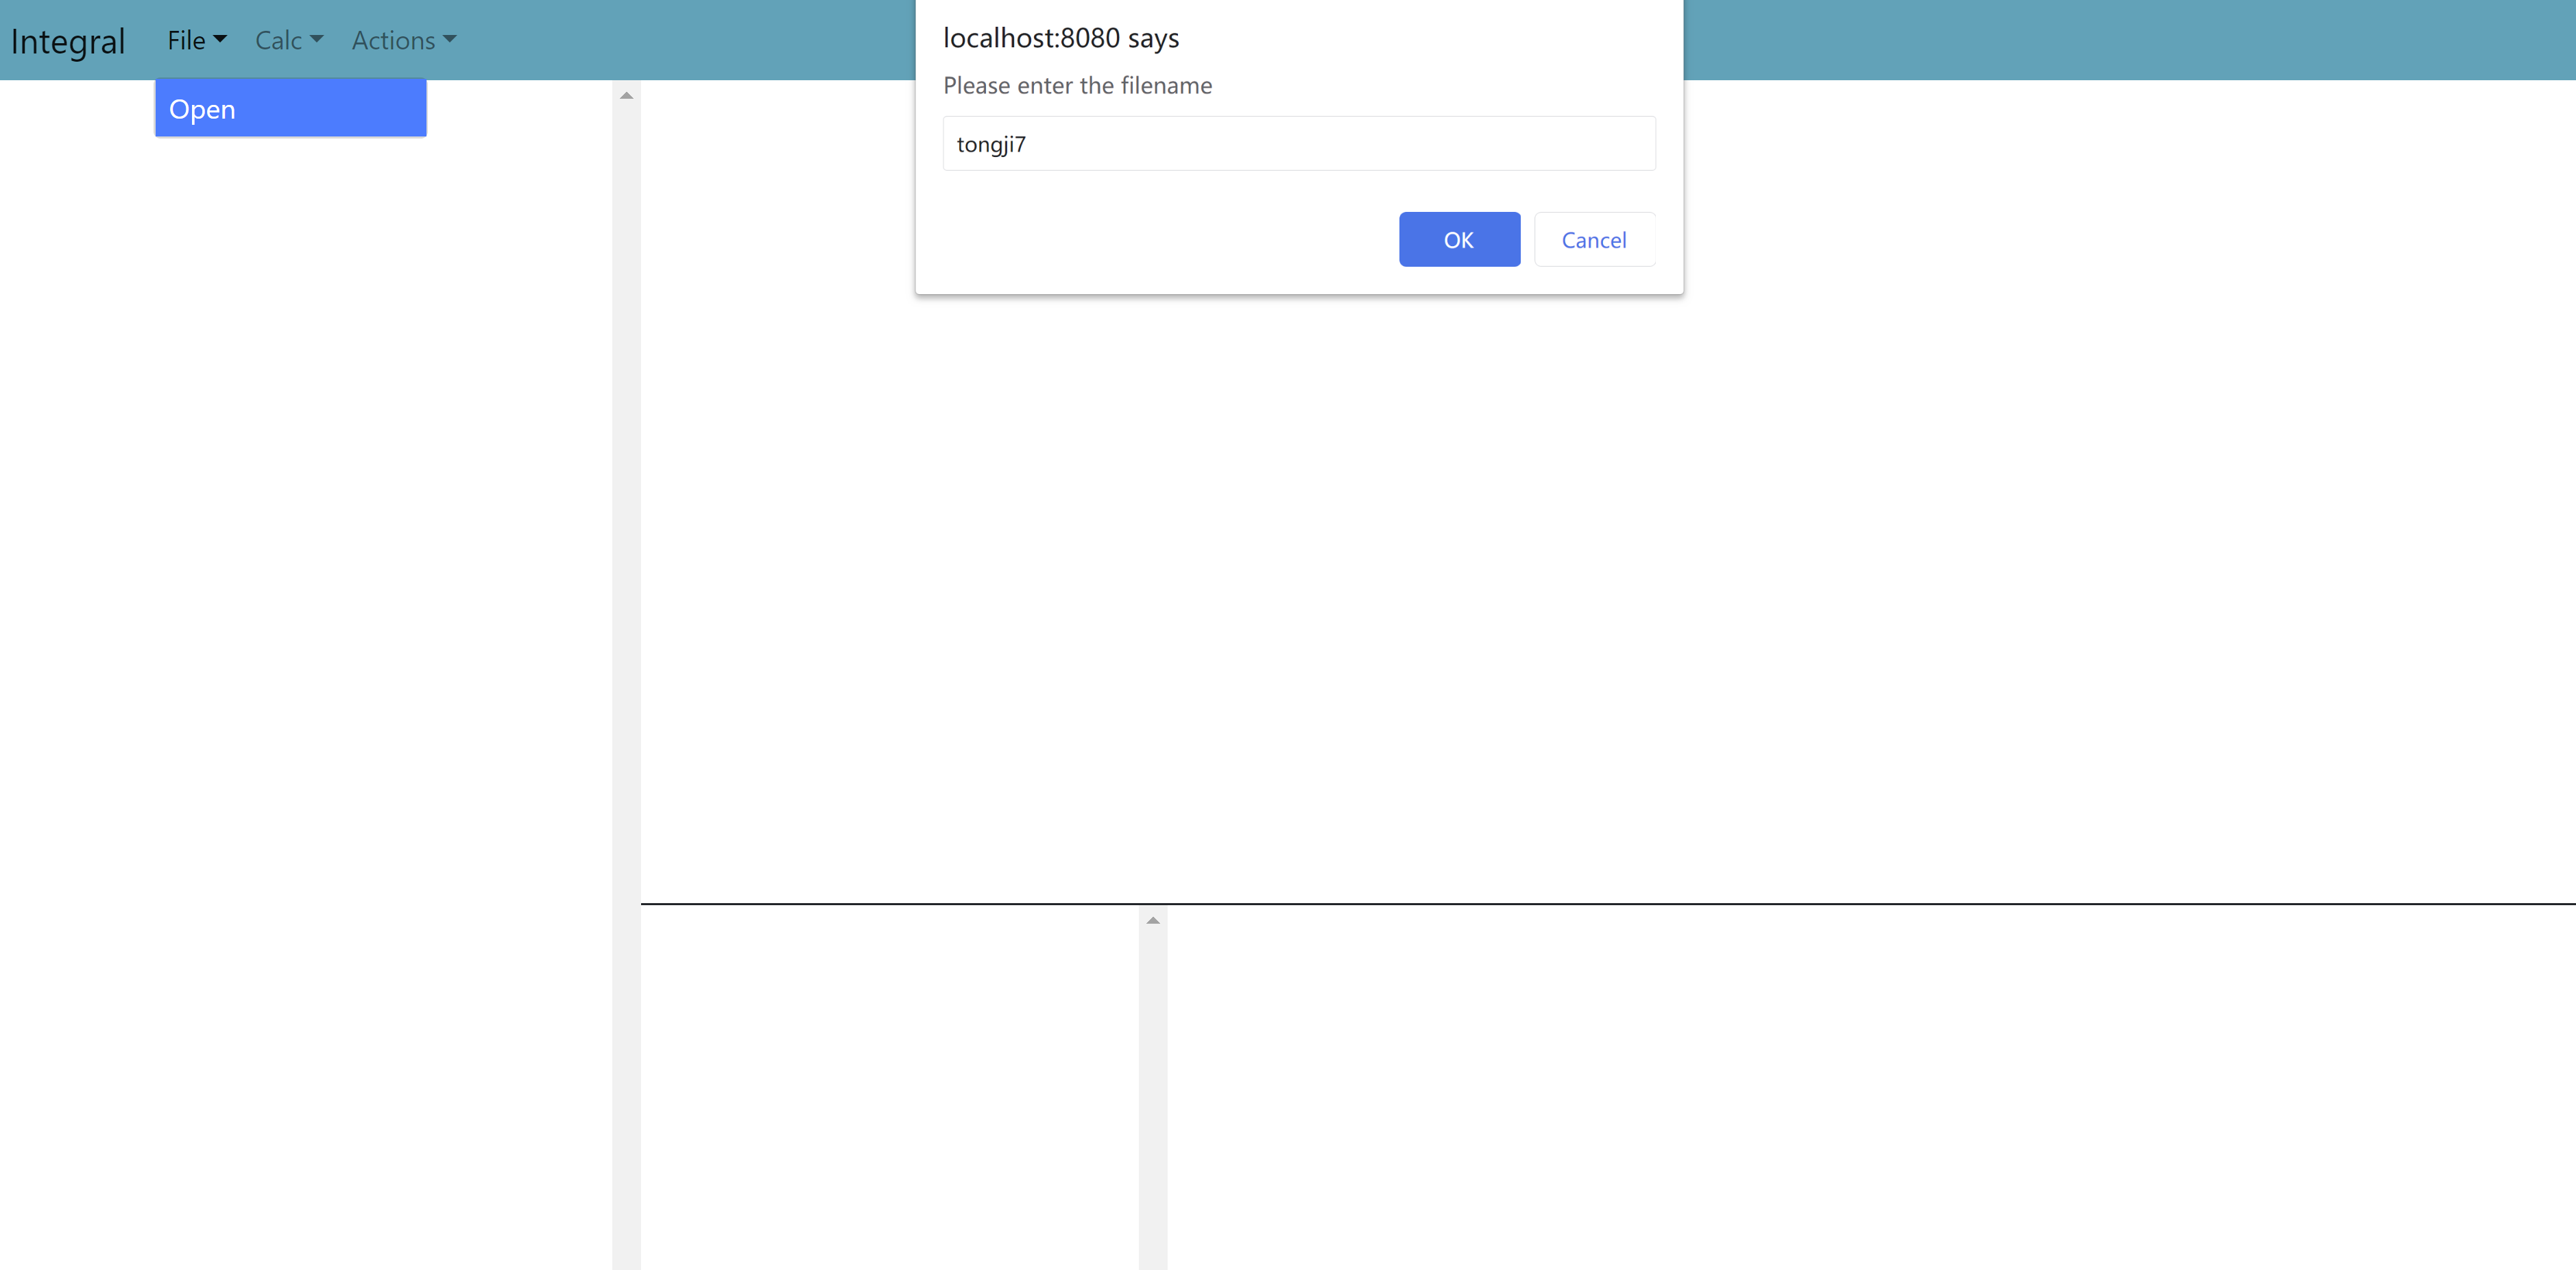
\includegraphics[width=14.5cm, height=4cm]{3.png}
The page becomes like this:\\
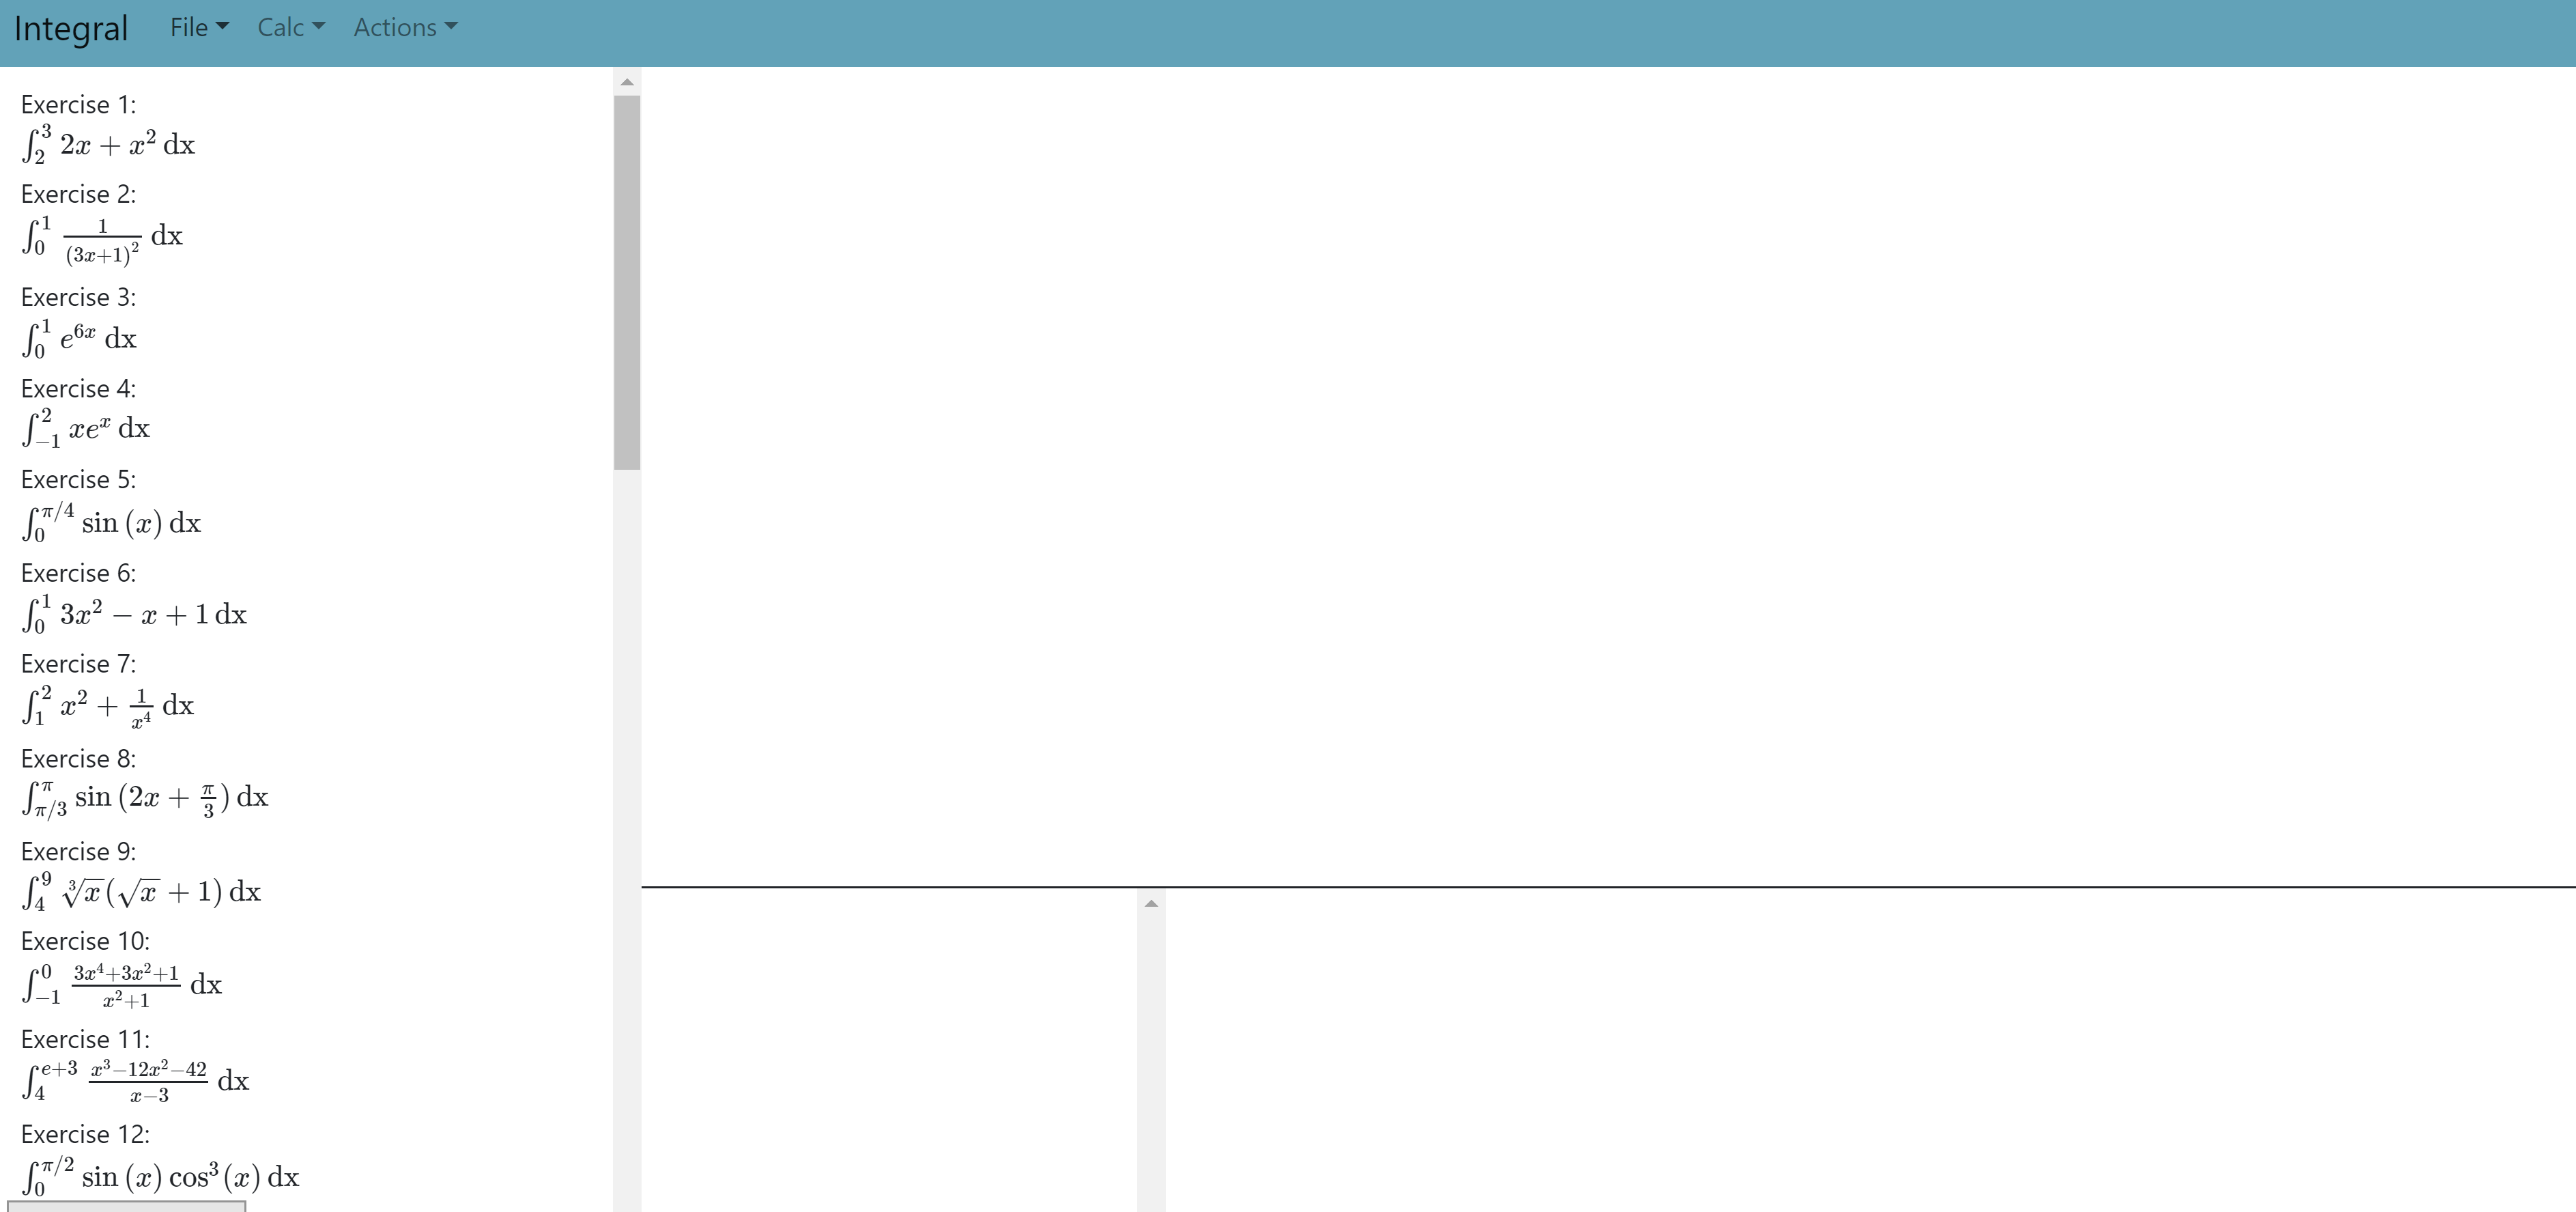
\includegraphics[width=13cm, height=7cm]{4.png}
We can see that the \rom{2} part are filled with all the integrals in the tongji7.json now.\\
\subsection{Select integral}
User can operate each integral in the json file by themselves, in order to do this, user need to click the integral in the \rom{2} part. If there are  no existing solution for the integral, the \rom{3} part becomes like this:\\
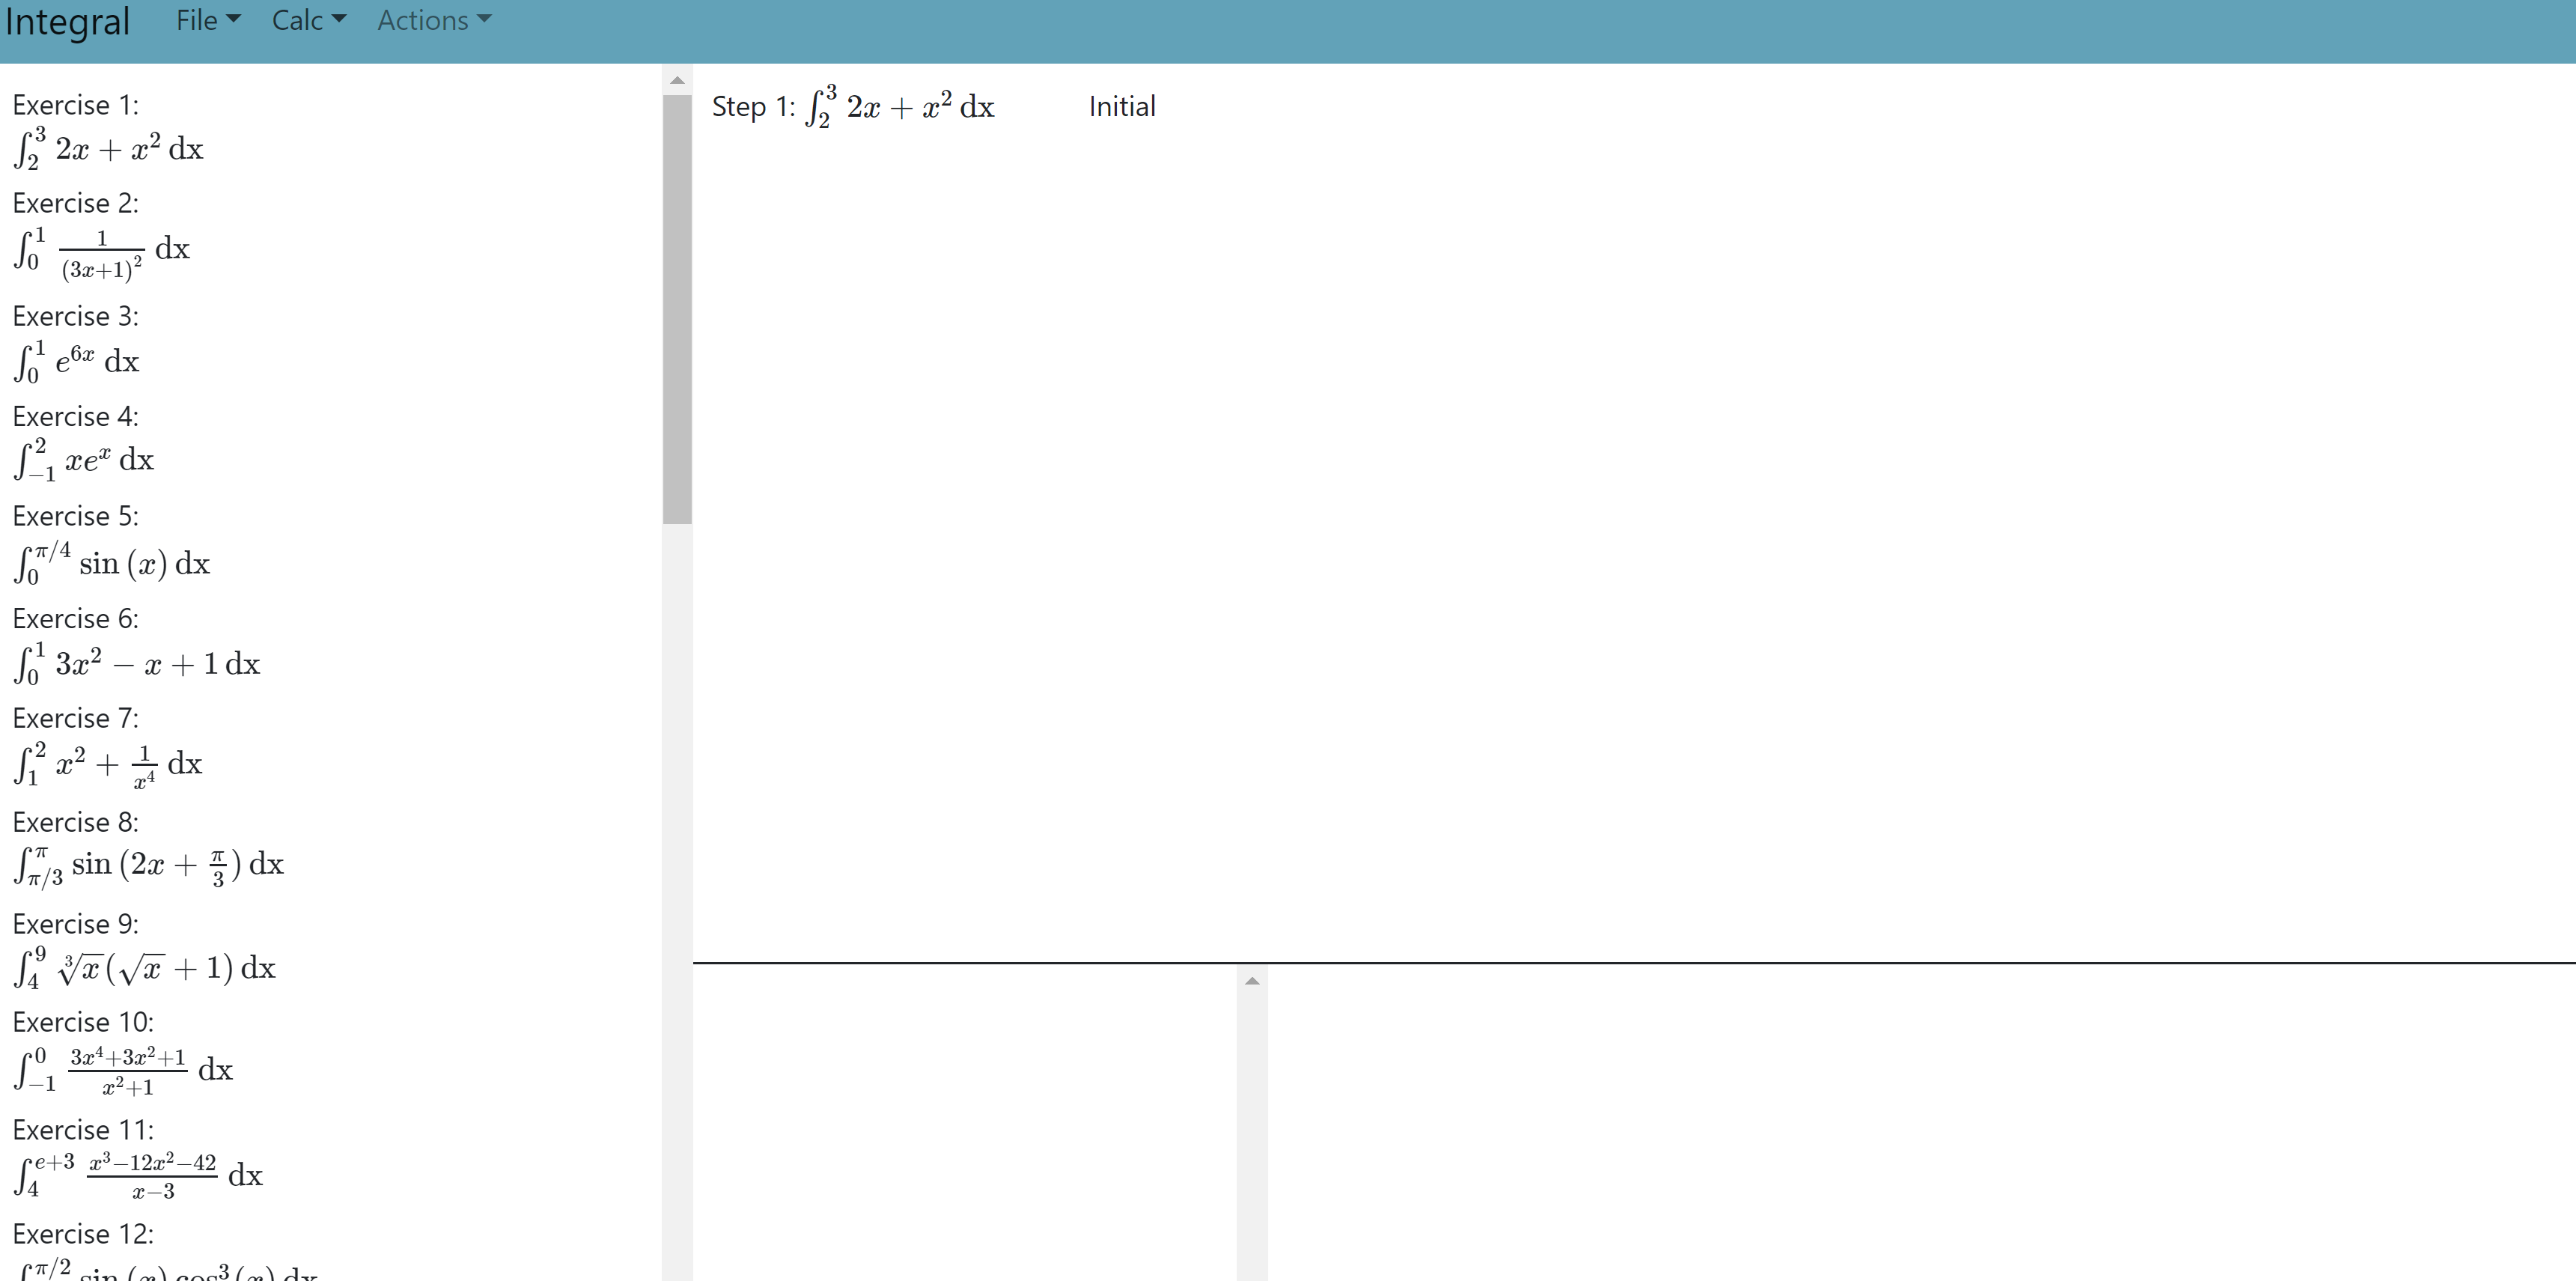
\includegraphics[width=13cm, height=7cm]{5.png}
If there are existing solution, \rom{3} will also display them together:\\
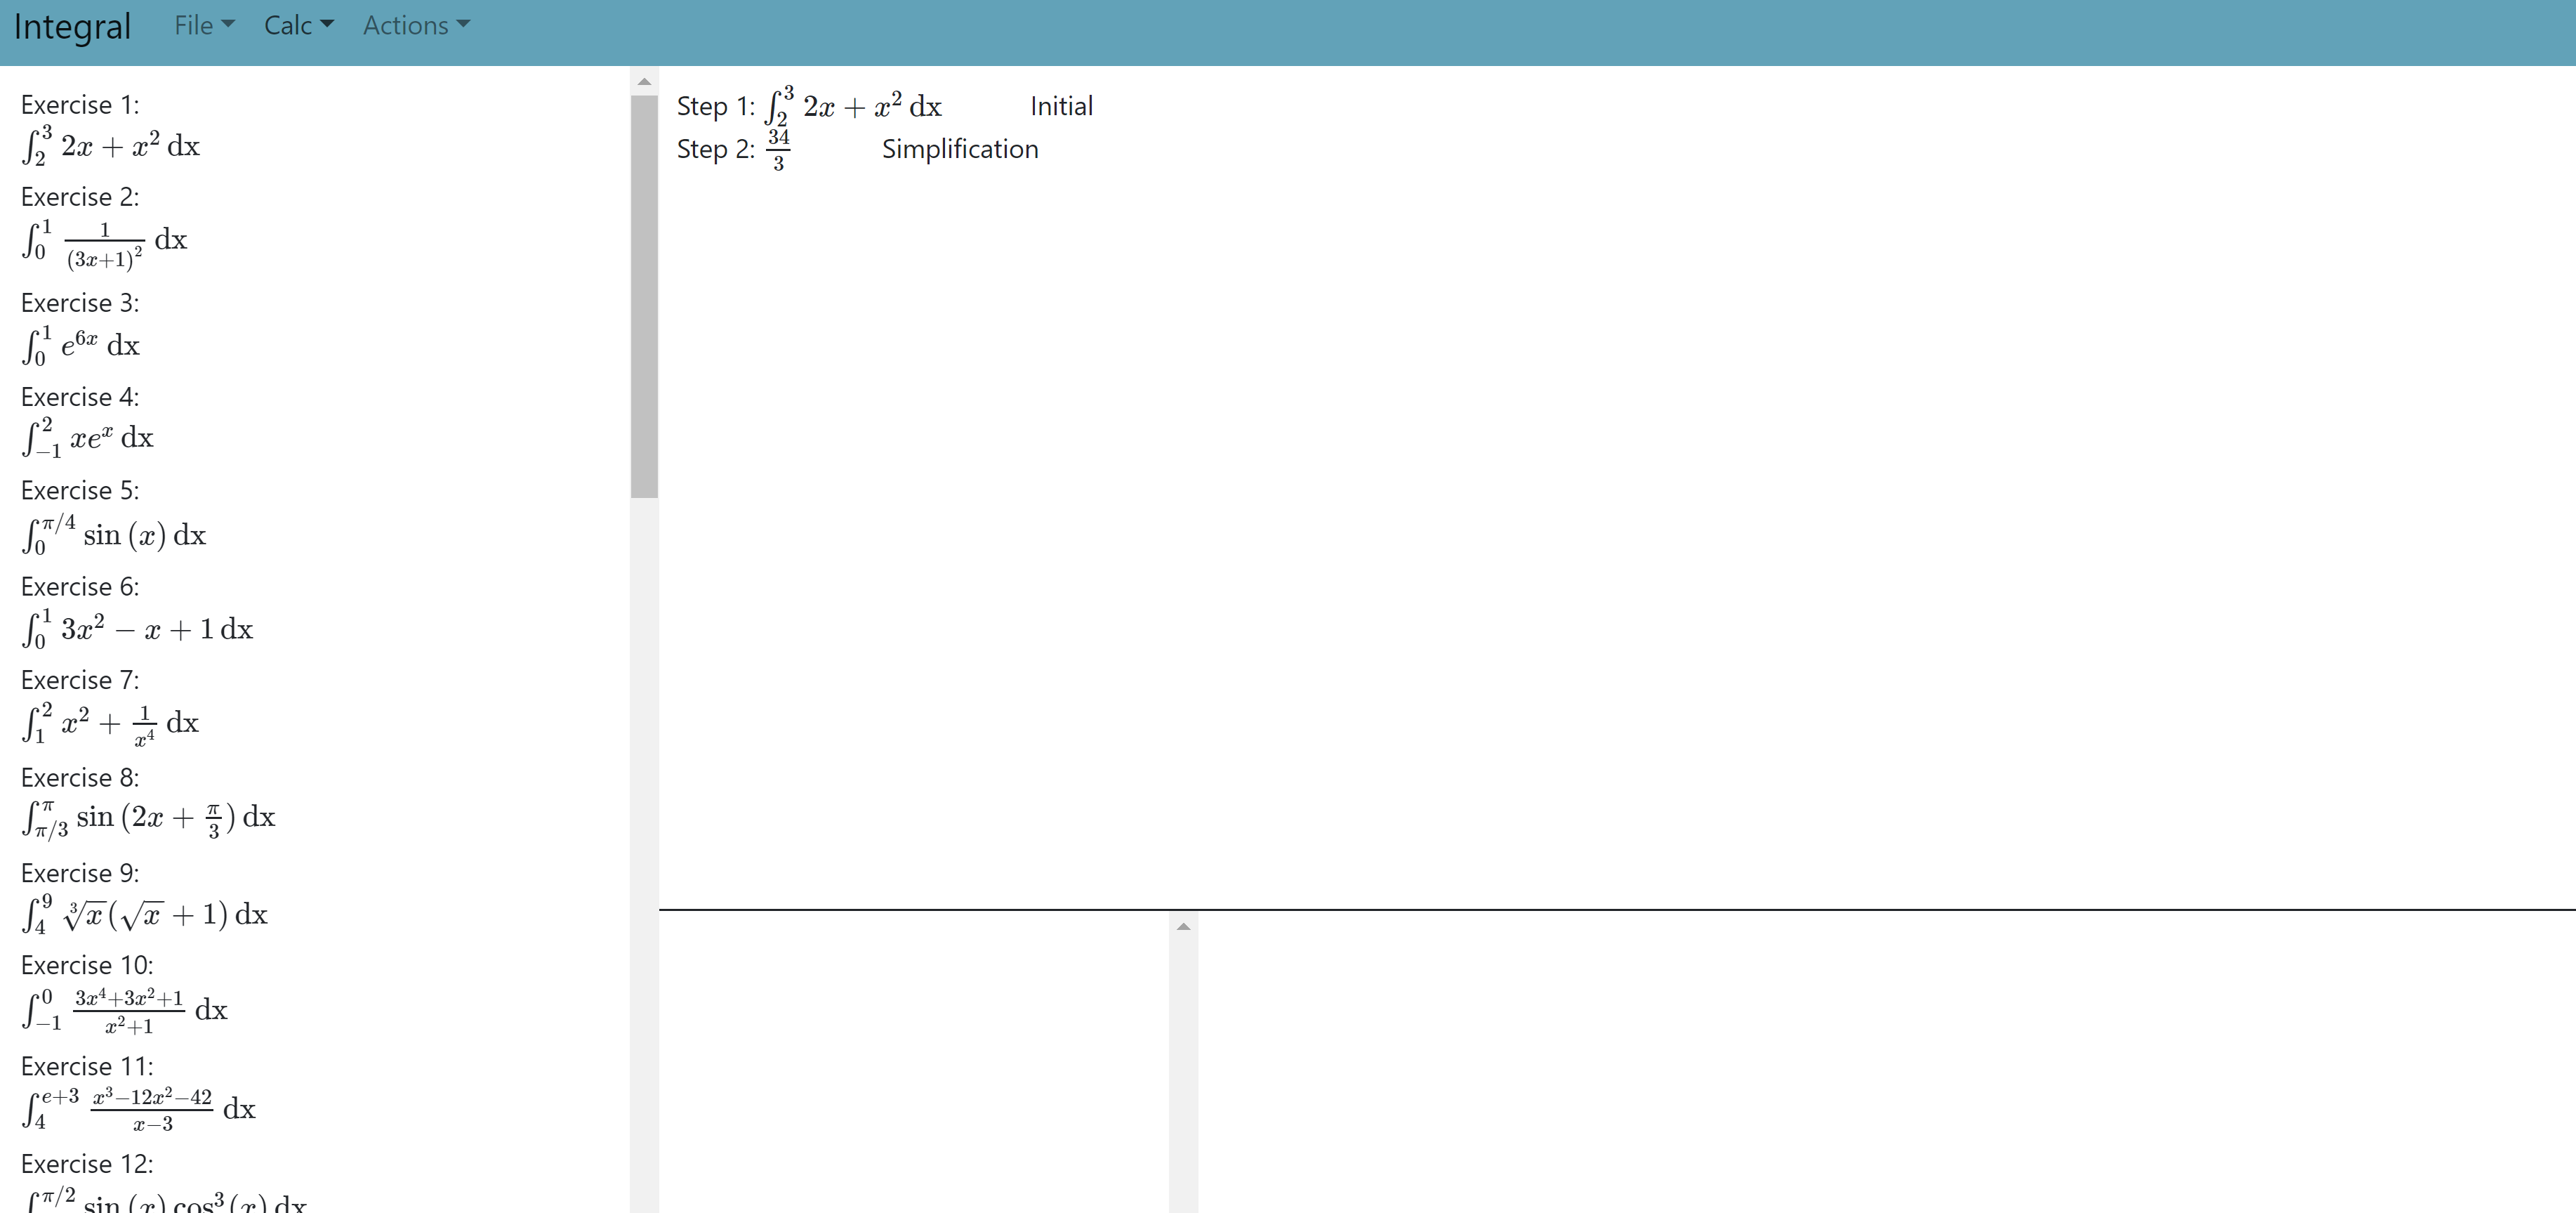
\includegraphics[width=13cm, height=7cm]{6.png}
\subsection{Utilities}
The following figure is a complete integration solution(./integral/example/MIT/2013.json exercise 1):\\
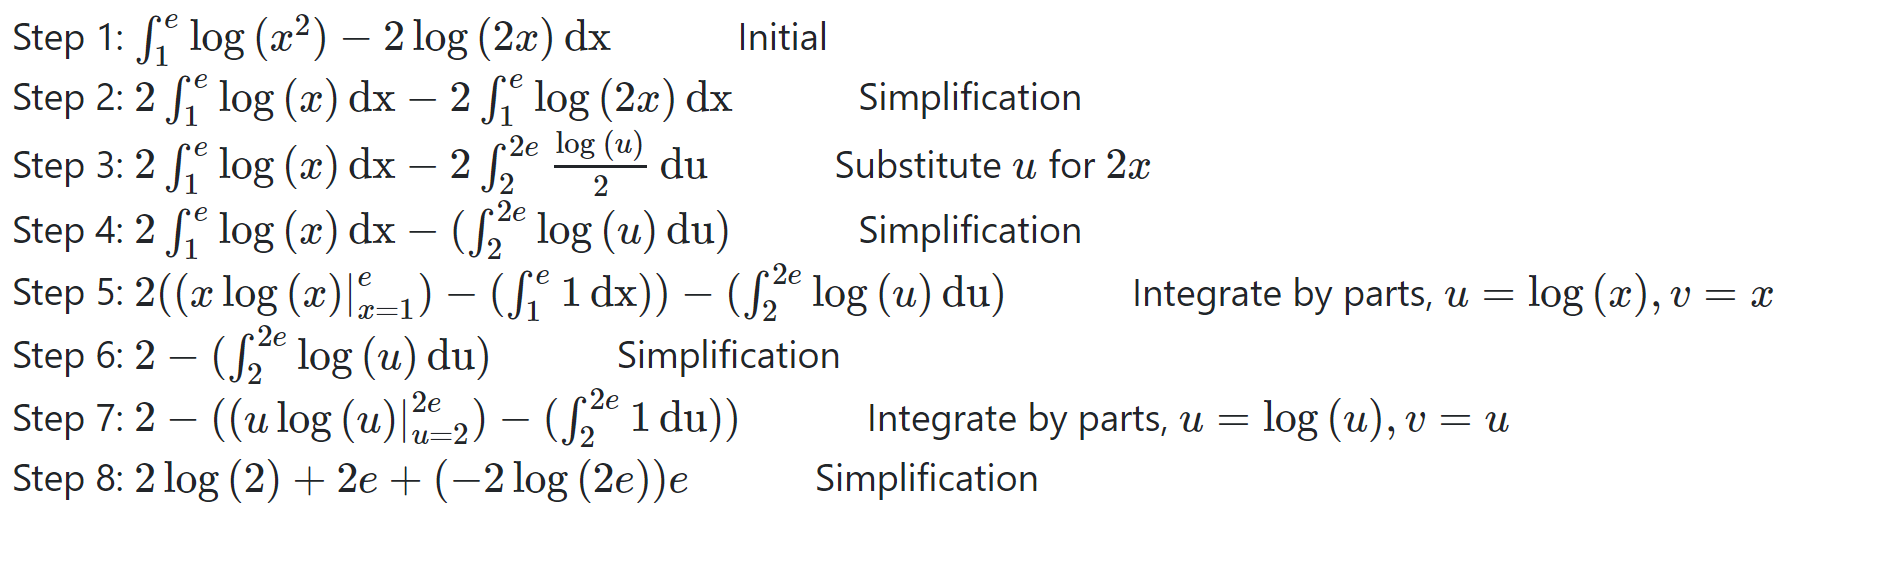
\includegraphics[width=14cm, height=6cm]{7.png}
We can observe how the integration works from the figure: Every line is a consequence by applying an integration rule(will introduce in 3.4) with a step identifier. So we provide several useful methods to operate with these steps in Calc menu.\\
If you apply a wrong rule, want to delete the current step and try again, can click the \colorbox{mygray}{Back} button, then the current step will be deleted.\\
If there is an exsiting solution for the selected integral in the json file, you want to do by yourself or try nother solutions, you may click the \colorbox{mygray}{Restart} button, all the steps except the original problem will be cleared(Note that they are not really deleted in the json file).\\
If you restart an integration and get trouble in some steps, you may want to refer to the existing solution. \colorbox{mygray}{Restore} button can help you to recover the problem solution existed in json file.\\
When you complete an integration, the solution is so beautiful that you may want to record it in the json file, then you can click the \colorbox{mygray}{Save} button to save the solution in the json file(Note that the previous solution will be replaced if it exists).
\subsection{Integration Rules}
The left part of the tutorial will focus on the integration rules. There are 9 rules will be discussed. We know that there is not only one way to compute an definite integral to correct answers. So while some rules can be applied automatically, such as Simplification or Rewrite fraction, others may need the user to provide some information. All the rule buttons are in menu Actions.
\subsubsection{Simplication}
When you want to rewrite an expression into an equivalent simpler form, you can consider the Simplification rule, this rule can automatically apply a common integration rule according to integral table on each integral and plug in the lower and upper bounds in the expression, separate the integral into the sum of several integrals whose body is a polynomial, eliminate abstract value in the range of integral bounds, and normalize a polynomial expression. For example, the tongji7 exercise 7:
\begin{center}
$\int_{1}^{2} x^2 + \frac{1}{x^4} dx$
\end{center}
Assume we solve this integral by hand, first maybe linearize the integral:
\begin{center}
$\int_{1}^{2} x^2 dx + \int_{1}^{2} \frac{1}{x^4} dx$
\end{center}
Then use the integral table to integrate each integral, and plug the lower and upper bound to get the result value 3/8. The above three steps can be done by clicking the \colorbox{mygray}{Simplify} button.\\
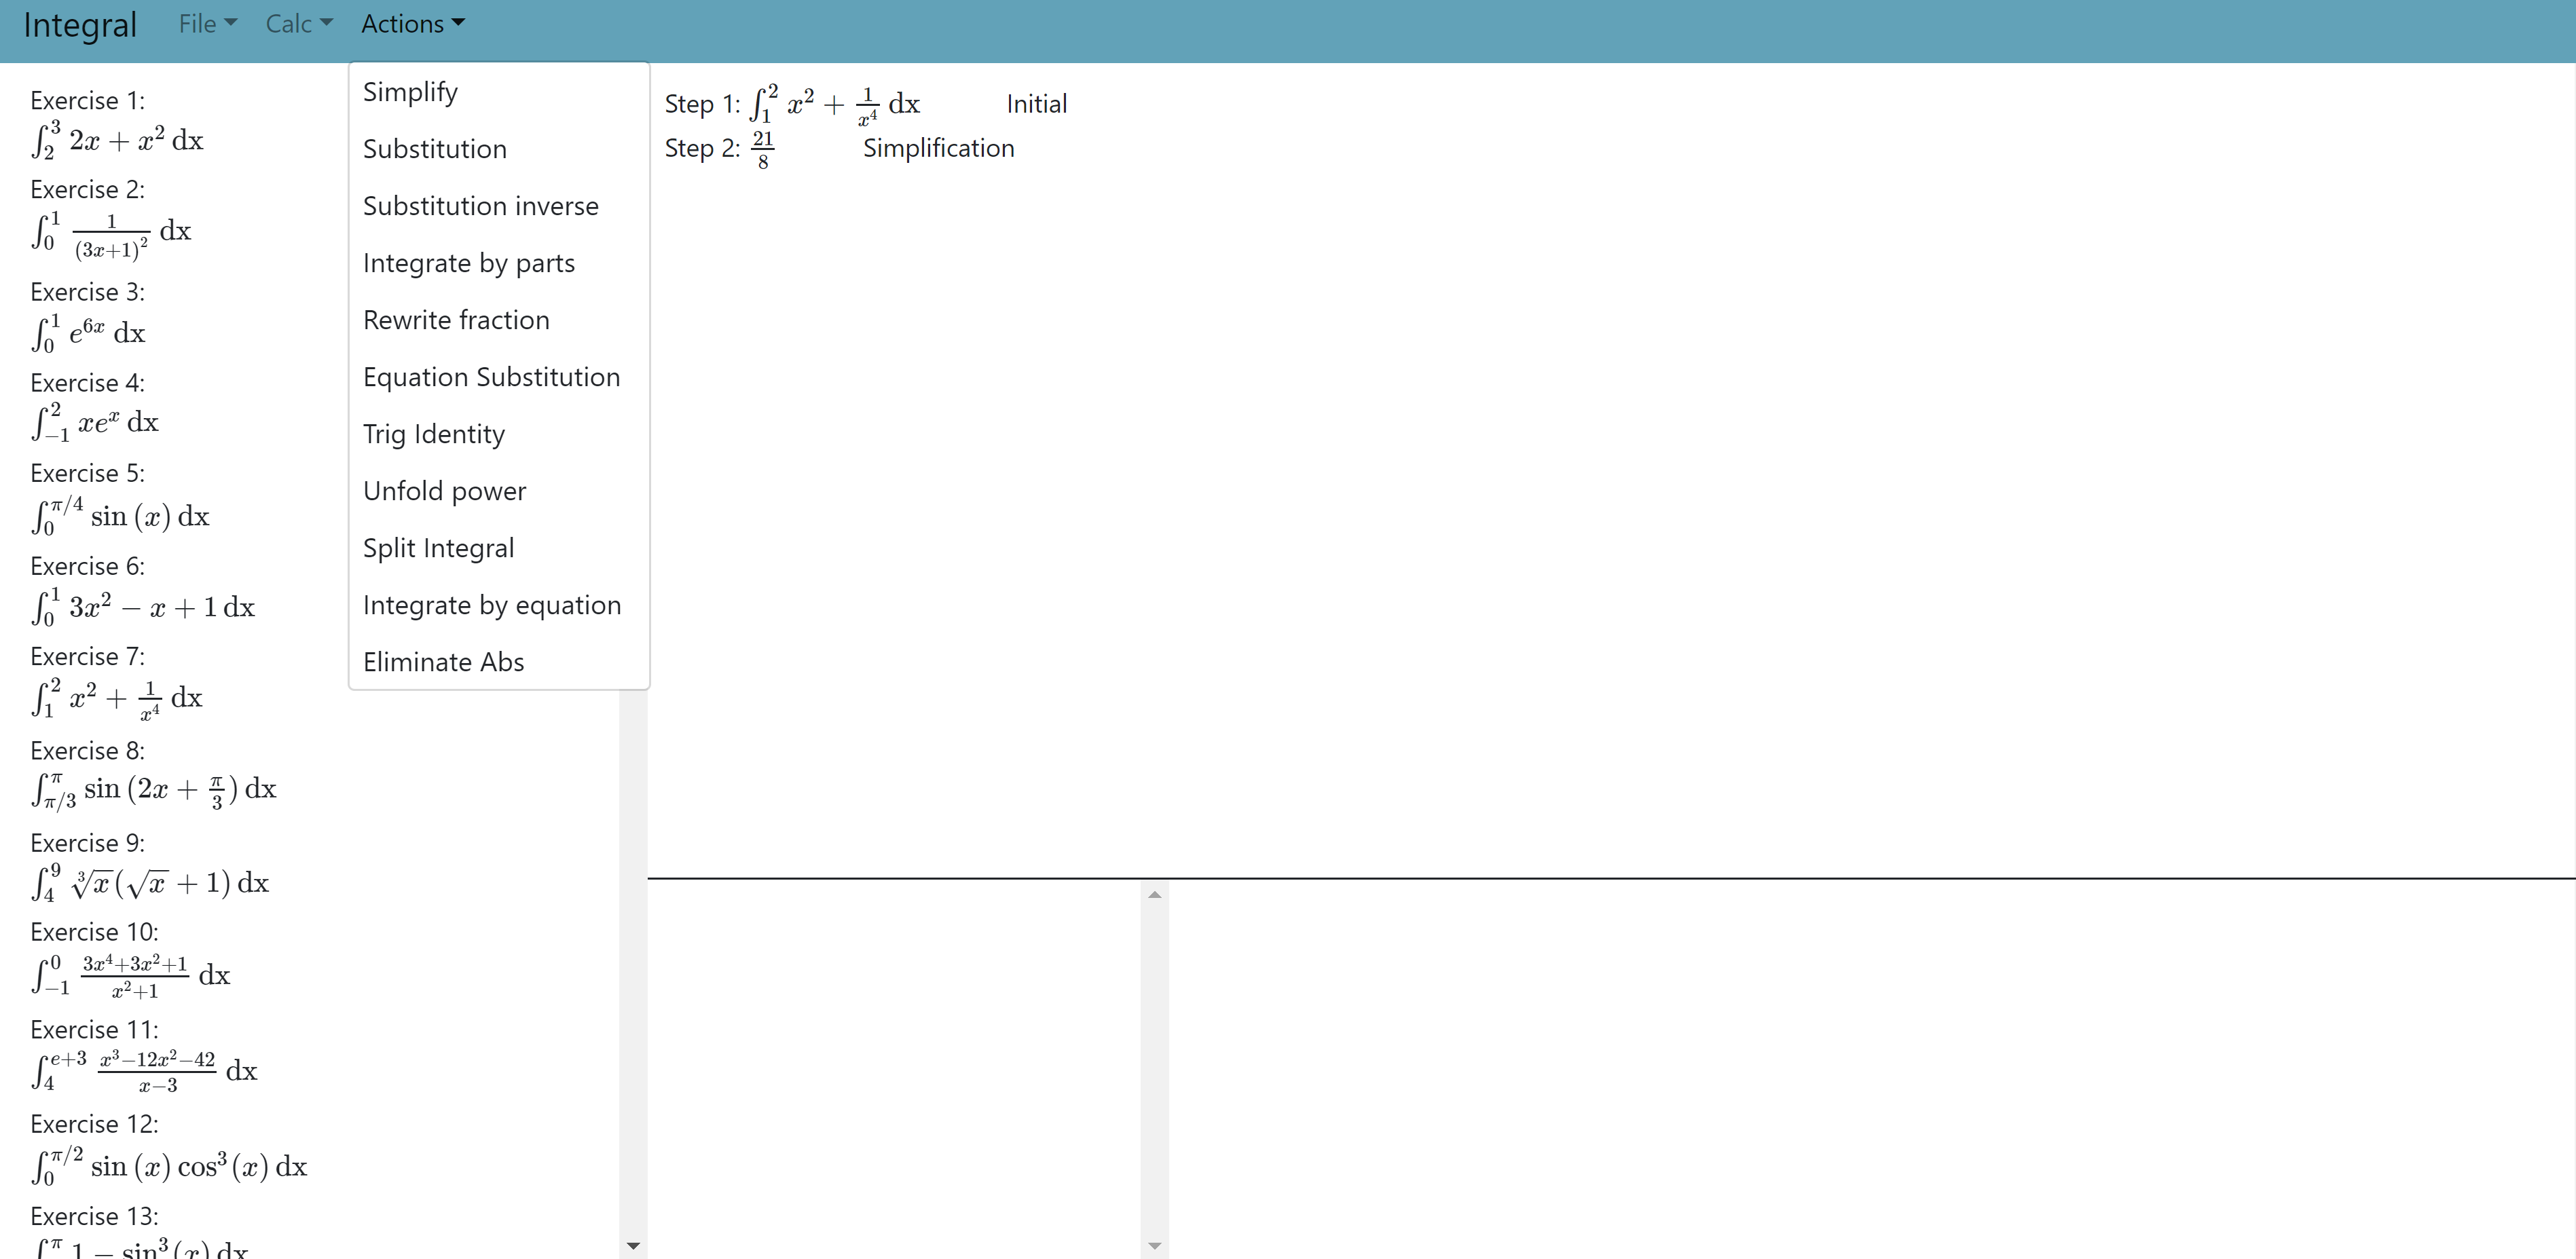
\includegraphics[width=13cm, height=7cm]{8.png}
\subsubsection{Forward substitution}
Substitution is common in integration. Sometimes you may need to substitute some f(x) in integration body by u, this is the case which the user should consider Forward Substitution rule. For example, the tongji7 exercise 3:
\begin{center}
$\int_{0}^{1} e^{6x} dx$
\end{center}
In order to do the substitution, you need to click the \colorbox{mygray}{Substitution} button. Then you can see that the \rom{4} displays all the integrals in the current step's expression(There are only one integral in this example). \\
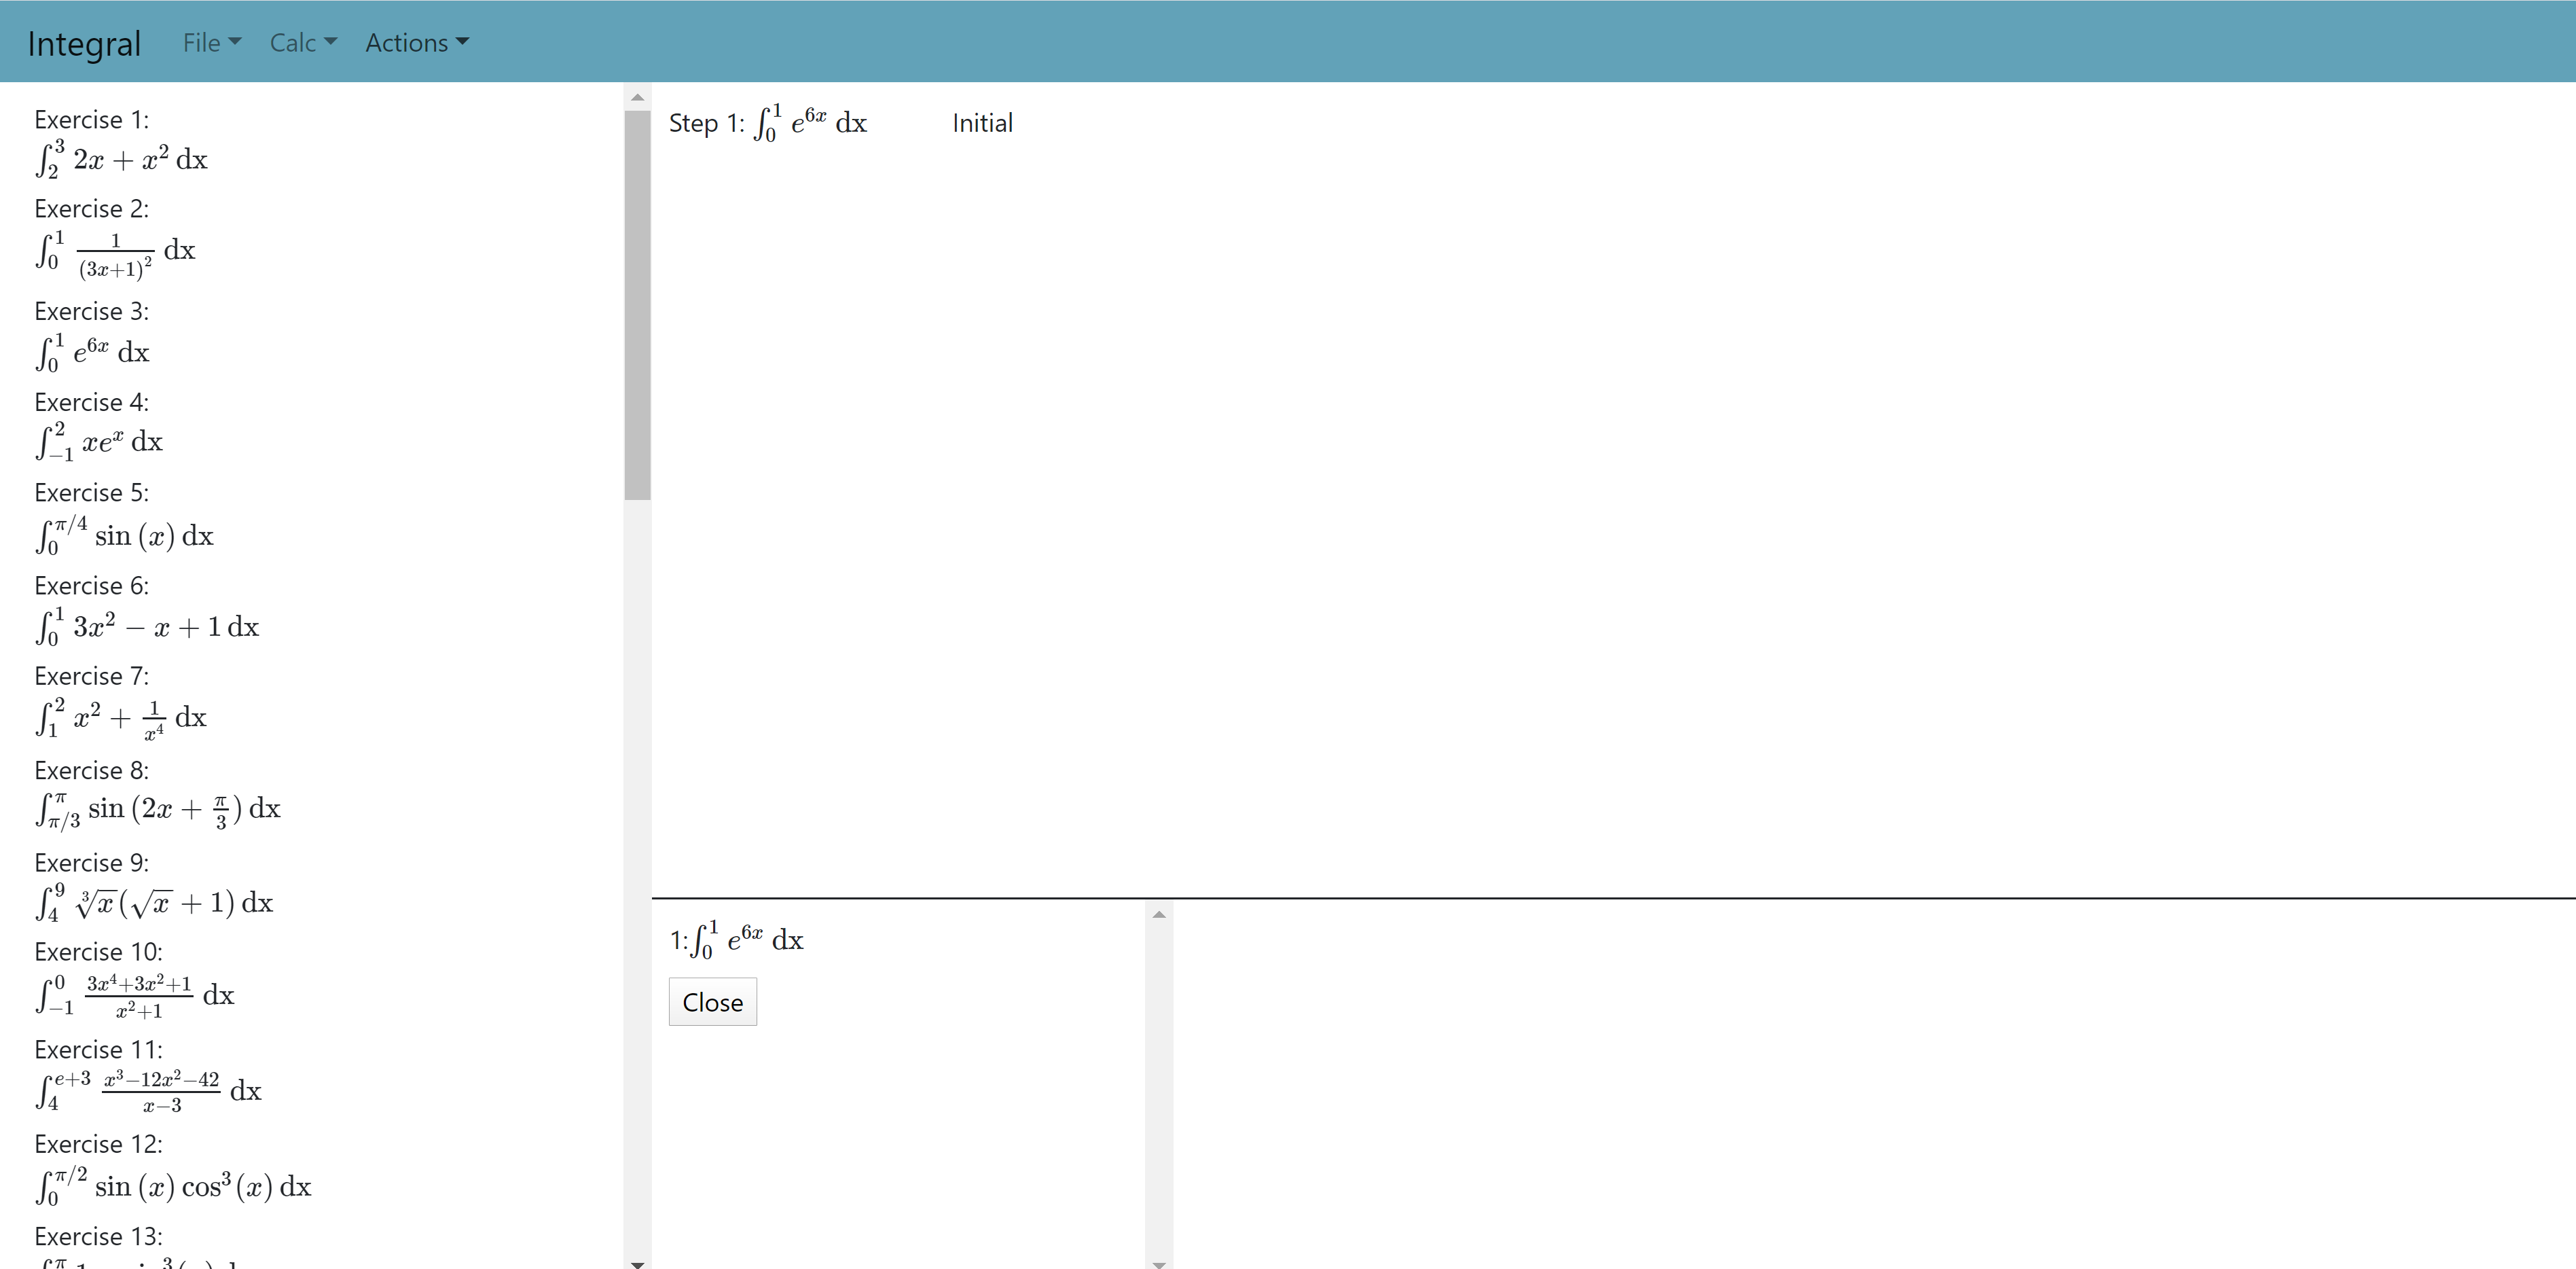
\includegraphics[width=13cm, height=7cm]{9.png}\\
You need to choose one integral you want to cope with(by clicking it). \rom{5} would display the necessary information you need to provide. The first text area represents the new integral variable will substitute in, the second text area represents the f(x) you want to be substituted. In this example, you can fill them with $u$ and $6*x$.\\\\
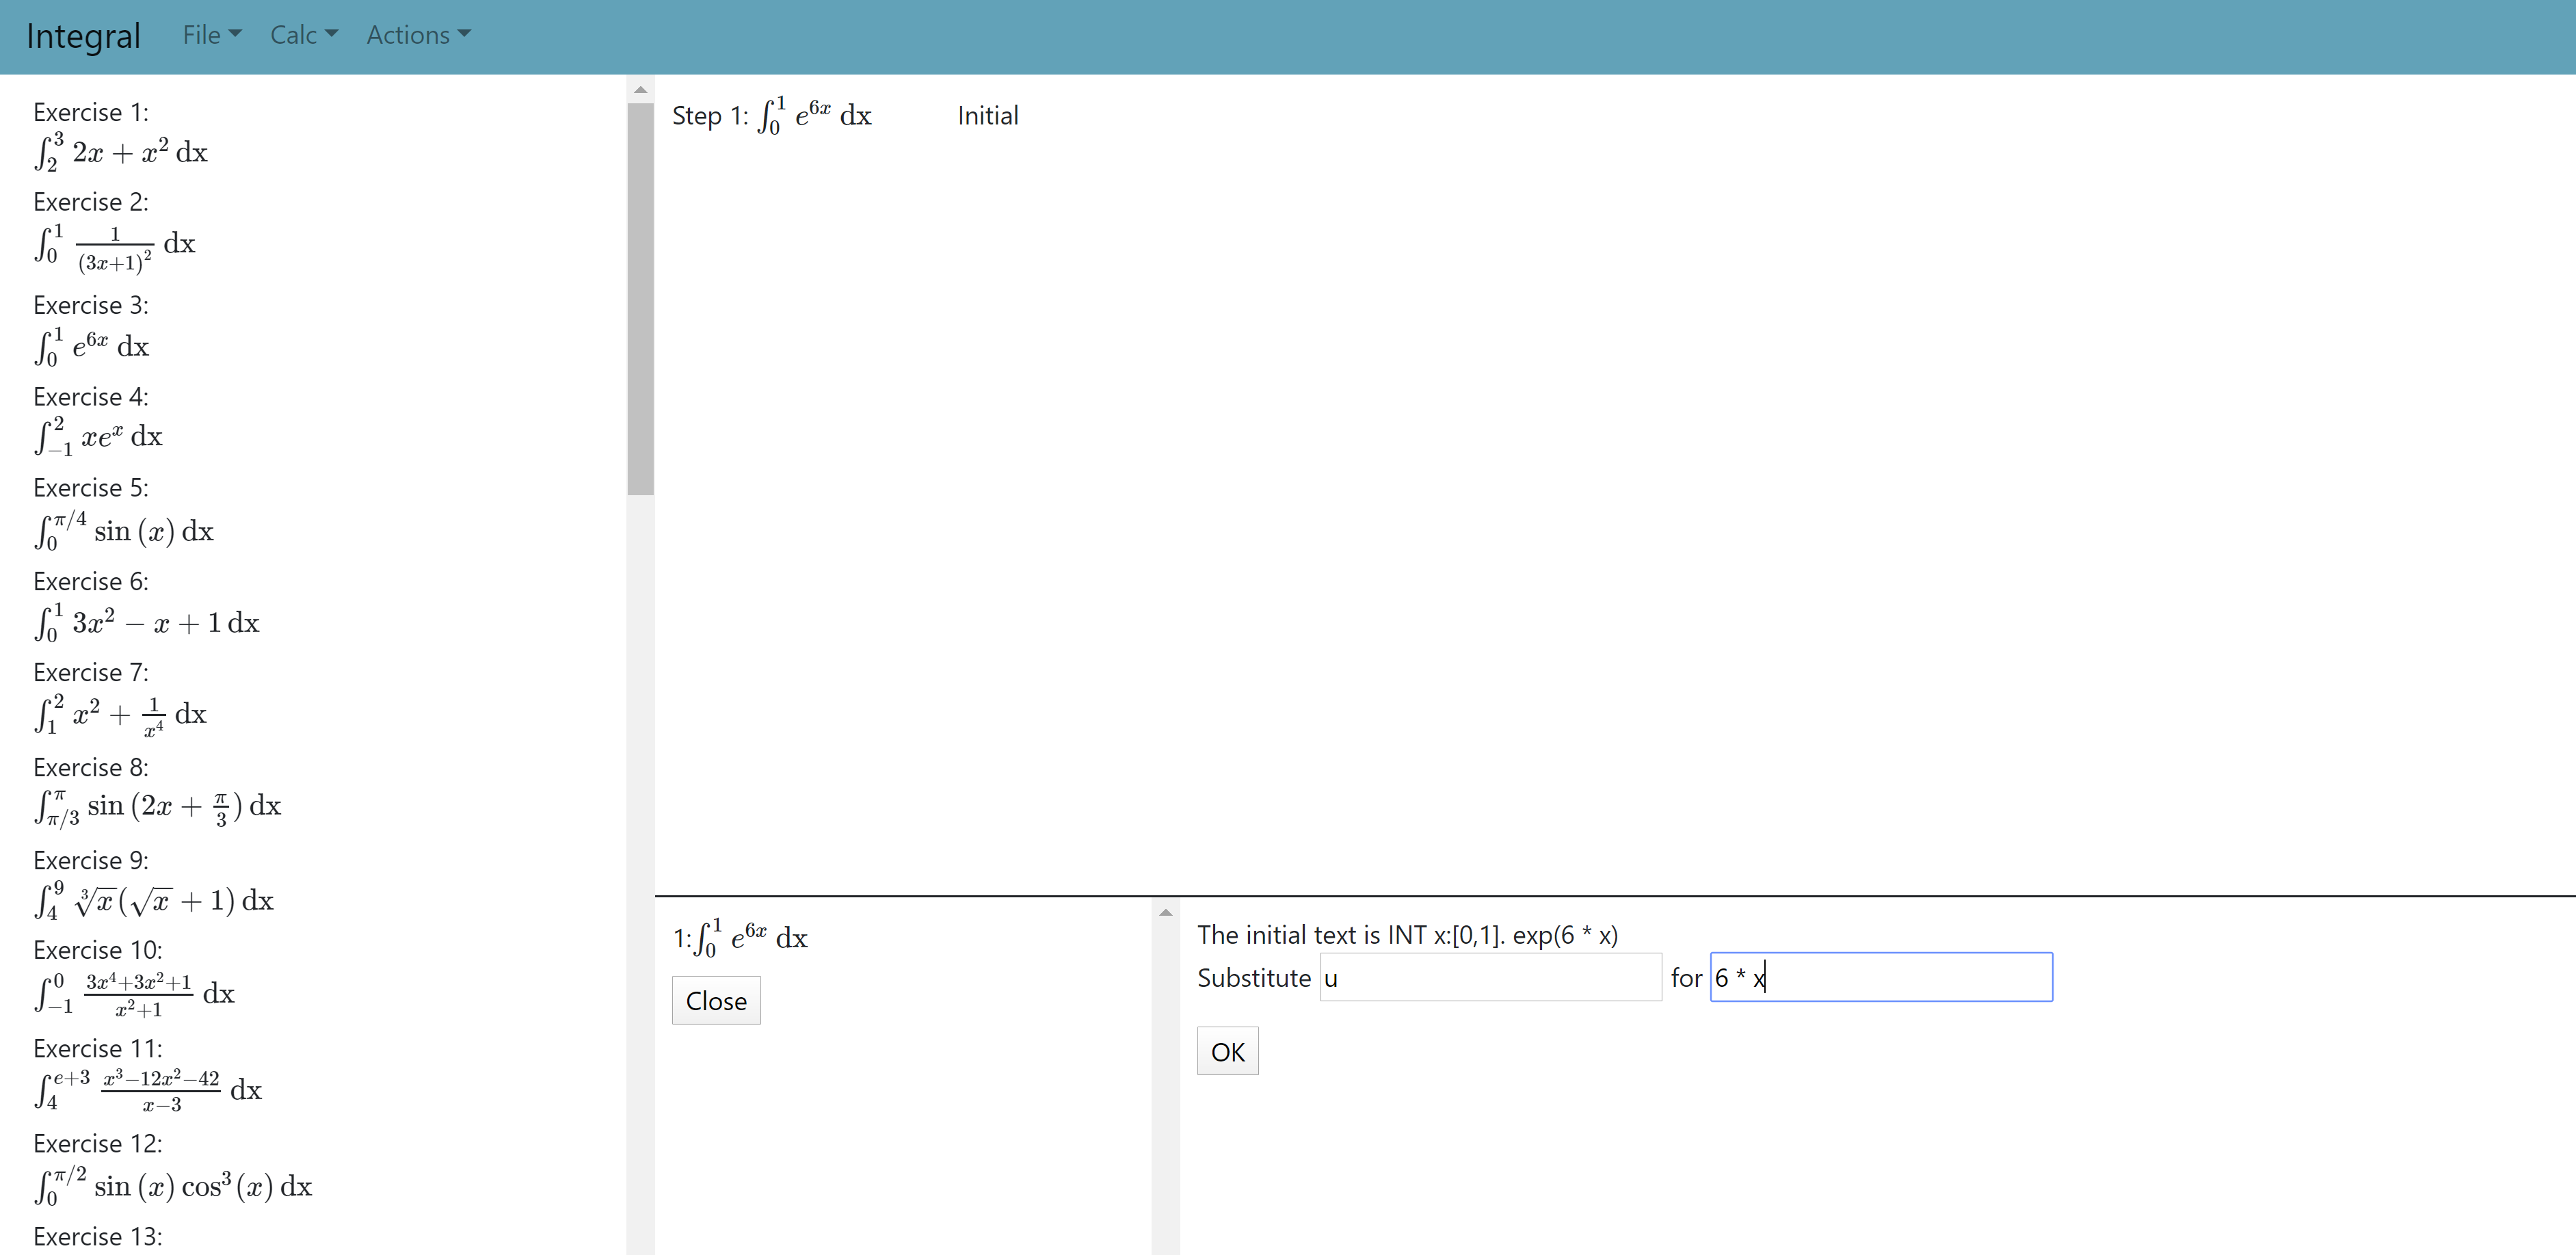
\includegraphics[width=13cm, height=7cm]{10.png}
By the time you complete these areas, you can click the \colorbox{mygray}{OK} button to finish this substitution. You can see \rom{4} and \rom{5} are cleared, and there is a new step in \rom{3}(We will not mention this in the following).\\
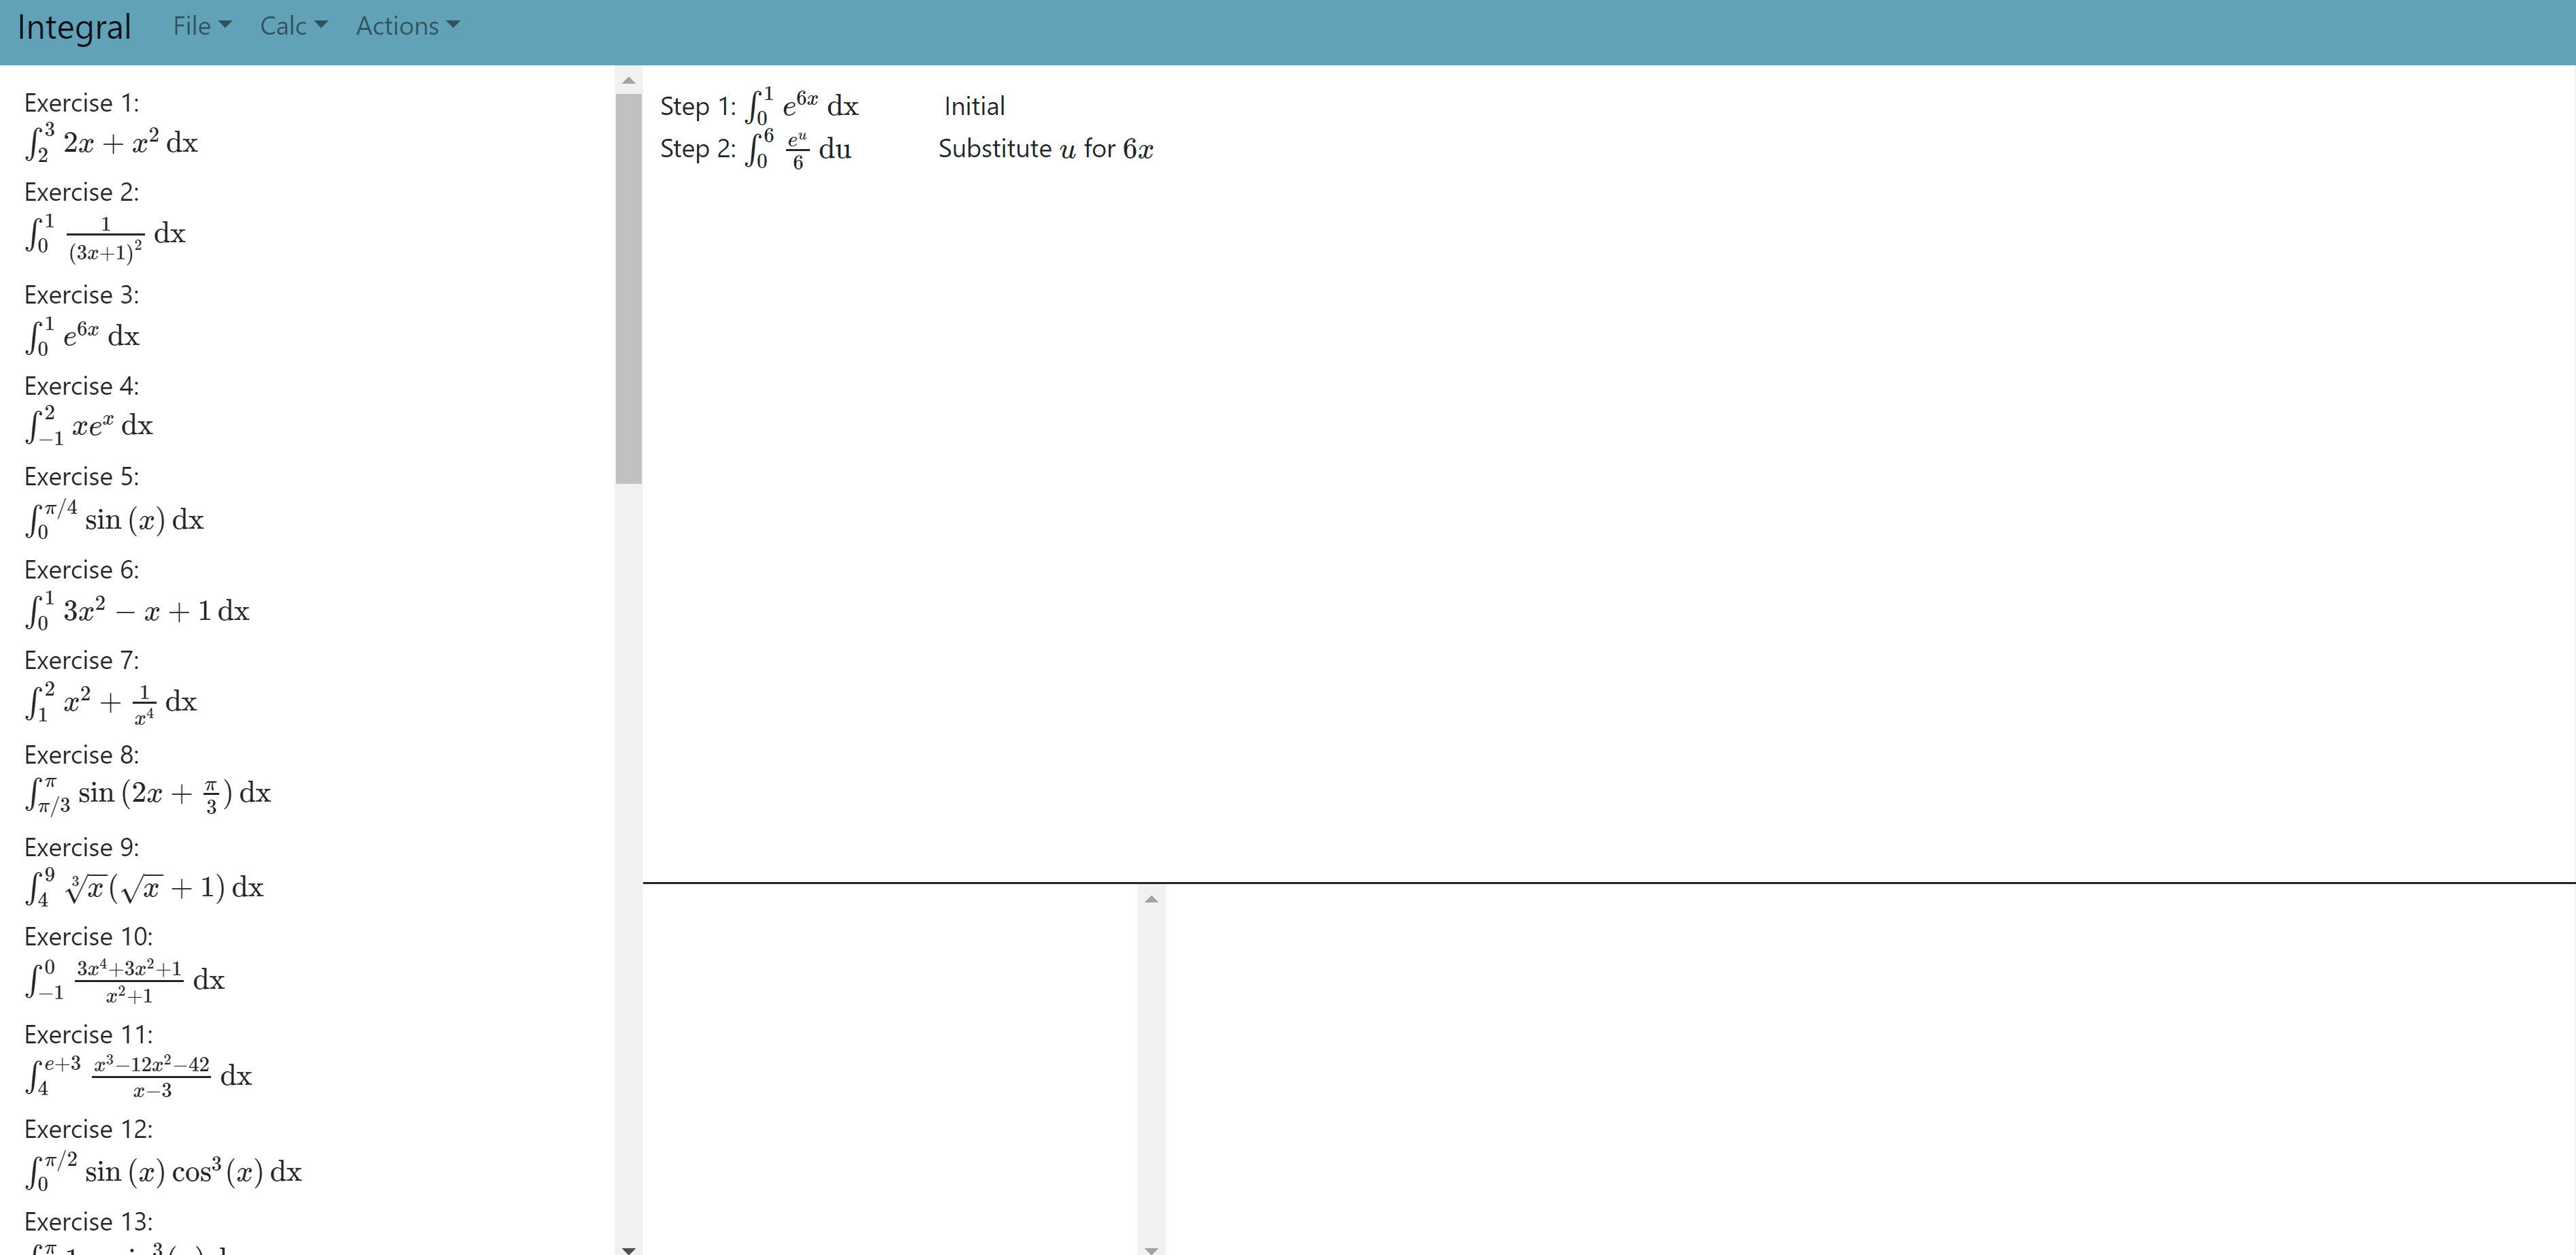
\includegraphics[width=13cm, height=7cm]{11.png}
\subsubsection{Backward substitution}
This is another substitution rule. In some cases, you may want to substitute x by some g(u) rather than substitute f(x) by a single u, for example, the tongji7 exercise 15:
\begin{center}
$\int_{0}^{1} \sqrt{1 - x^2} dx$
\end{center}
This time you can substitute x by something like sin(u) to simplify this problem. Click \colorbox{mygray}{substitution inverse} button, and click the integral you want to operate like in 3.4.2:\\\\
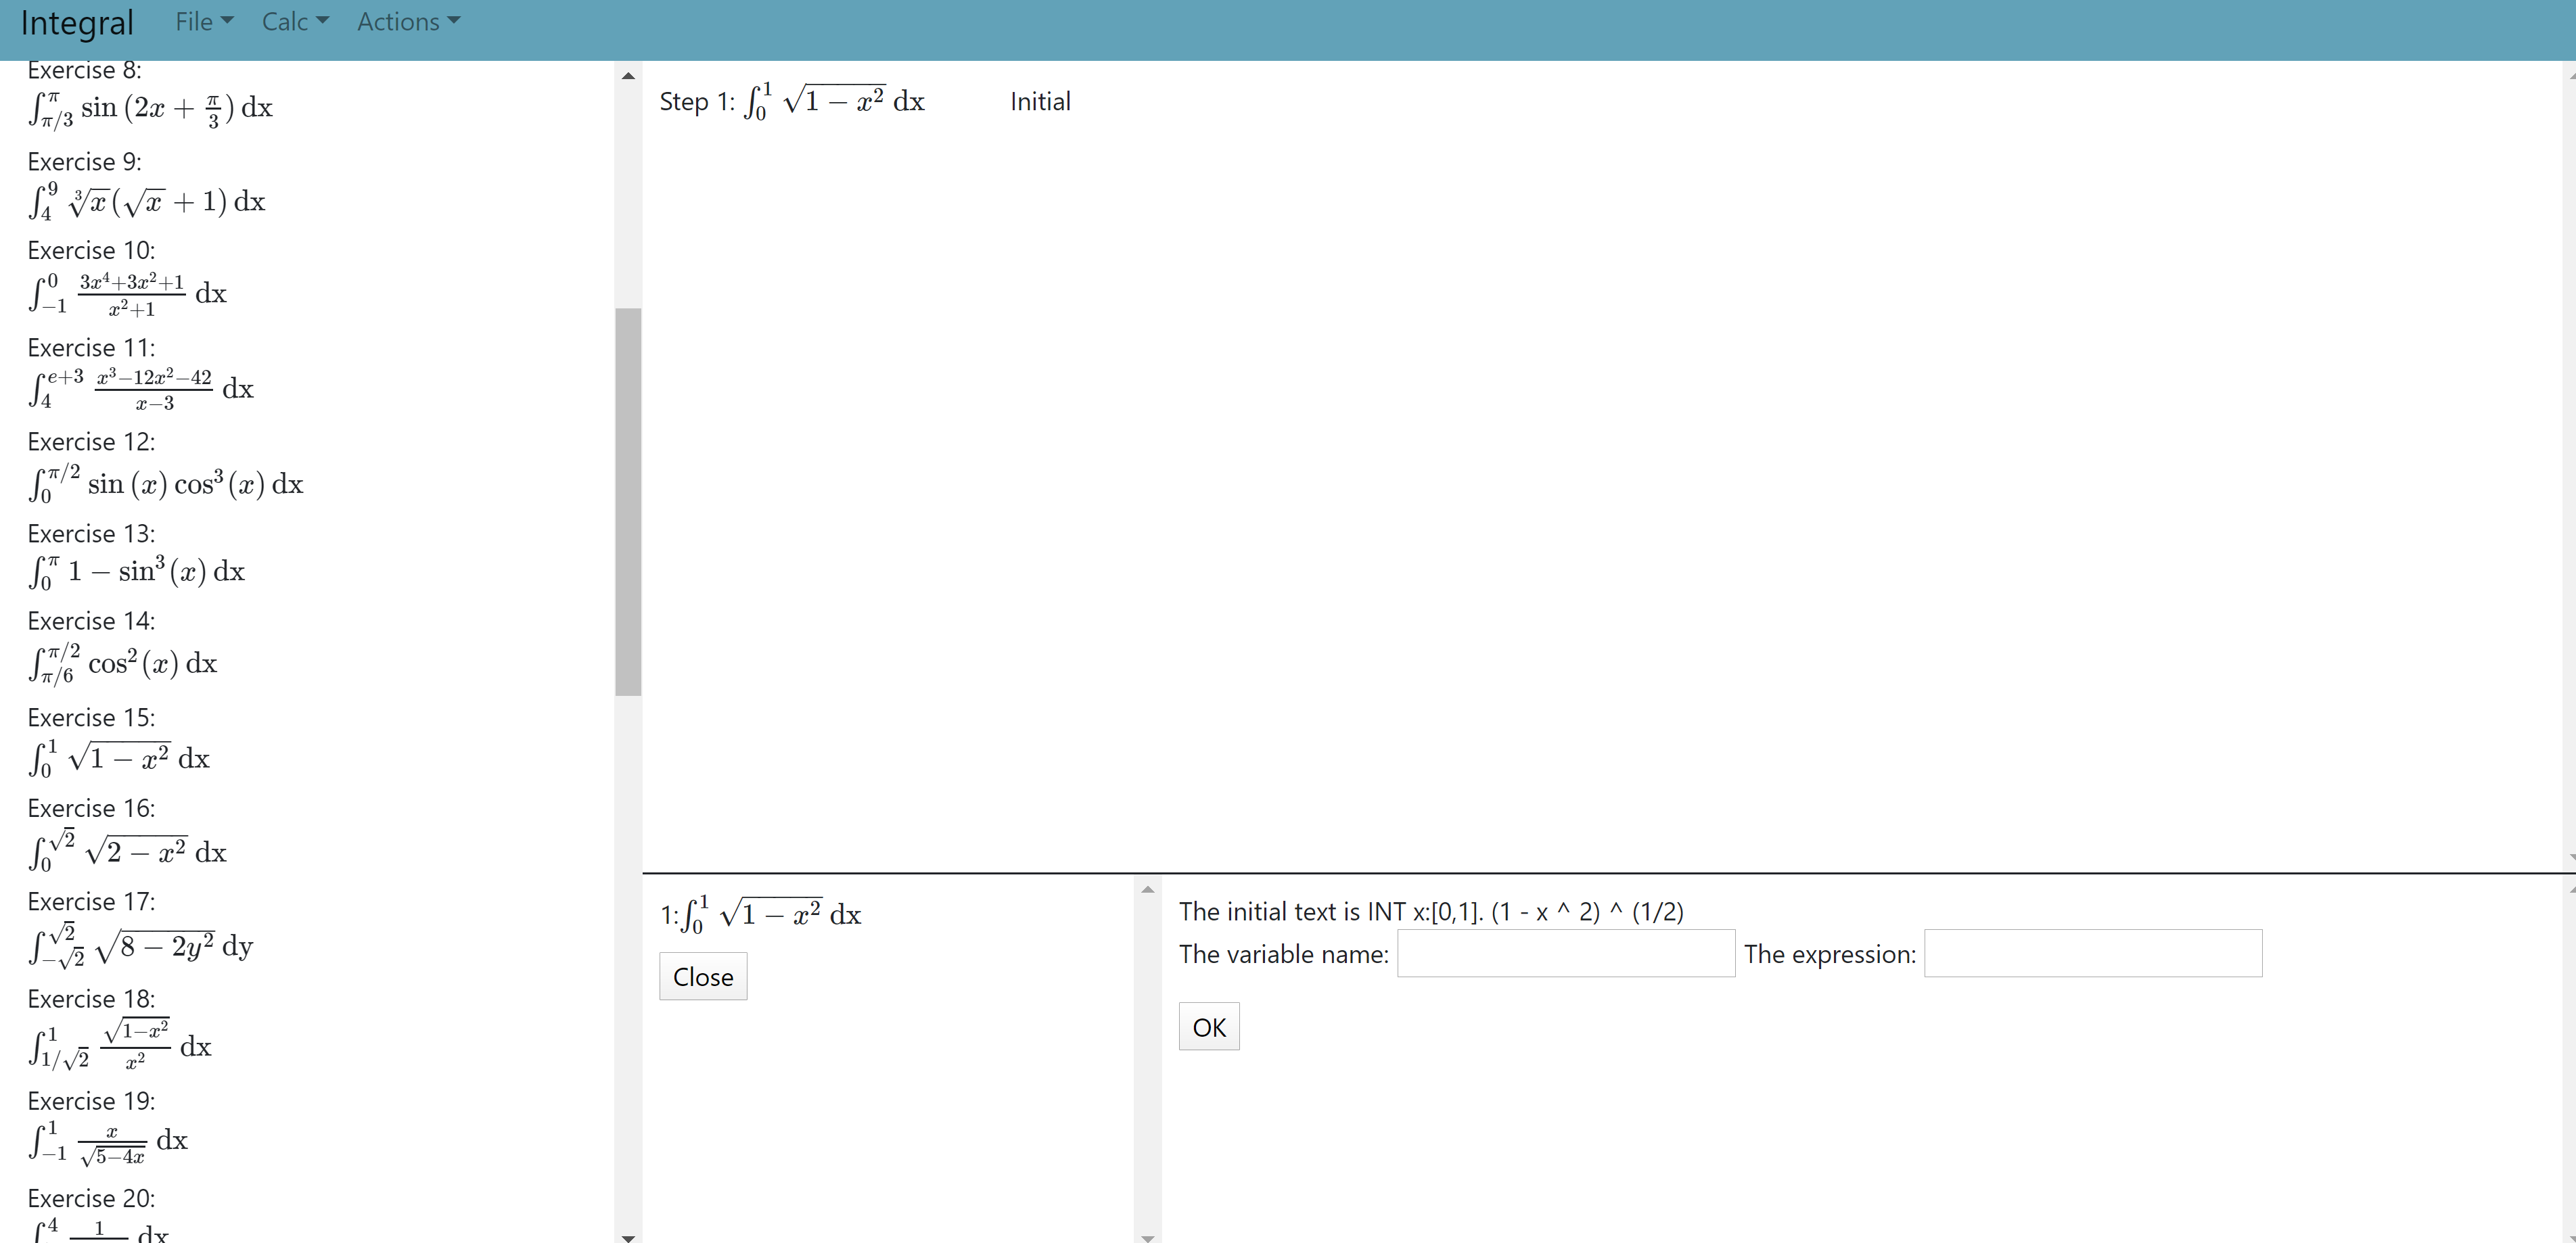
\includegraphics[width=13cm, height=7cm]{12.png}
Note that the text area meanings are different from 3.4.2. With the consideration that the integration variable will be substituted is fixed, so we don't need to tell HolPy. Instead, you should fill the first area with the new integration variable(because the $g(u)$ may contain other constant symbols), and write the $g(u)$ in the second. We fill them like this:\\\\
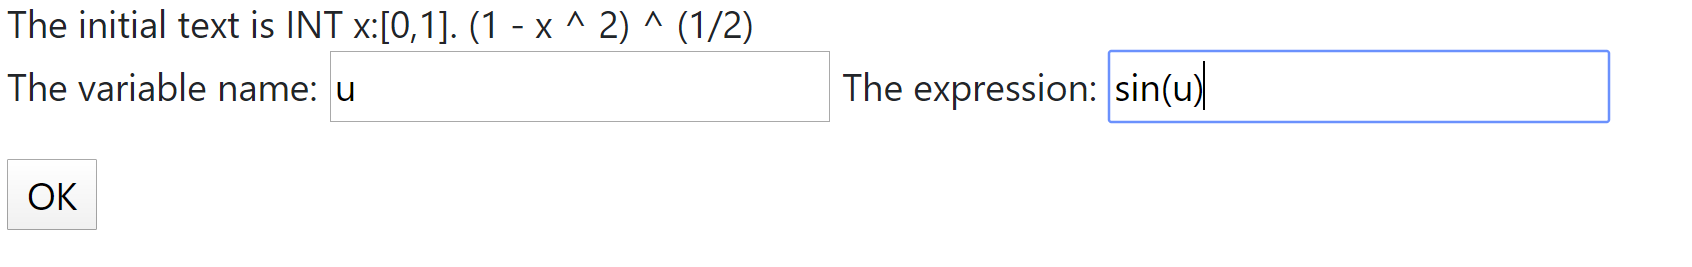
\includegraphics[width=13cm, height=3cm]{13.png}
Then the \rom{3} becomes:\\\\
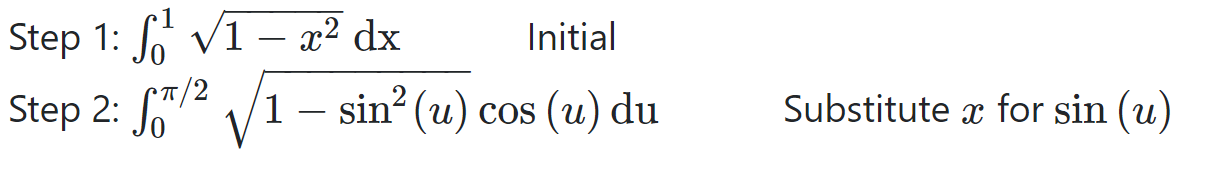
\includegraphics{30.png}
\subsubsection{Integrate by parts}
When the function body is a multiplication of variable and exponential function or trigonometric function, you may consider apply Integrate by parts rule. For instance, the tongji7 exercise 4:
\begin{center}
$\int_{0}^{1} xe^{x} dx$
\end{center}
Obviously, if we rewrite the body $xe^{x} dx$ to $x de^{x}$, the problem will be simpler. Click the \colorbox{mygray}{Integrate by part} button, and choose integral as before, the interface will become:\\
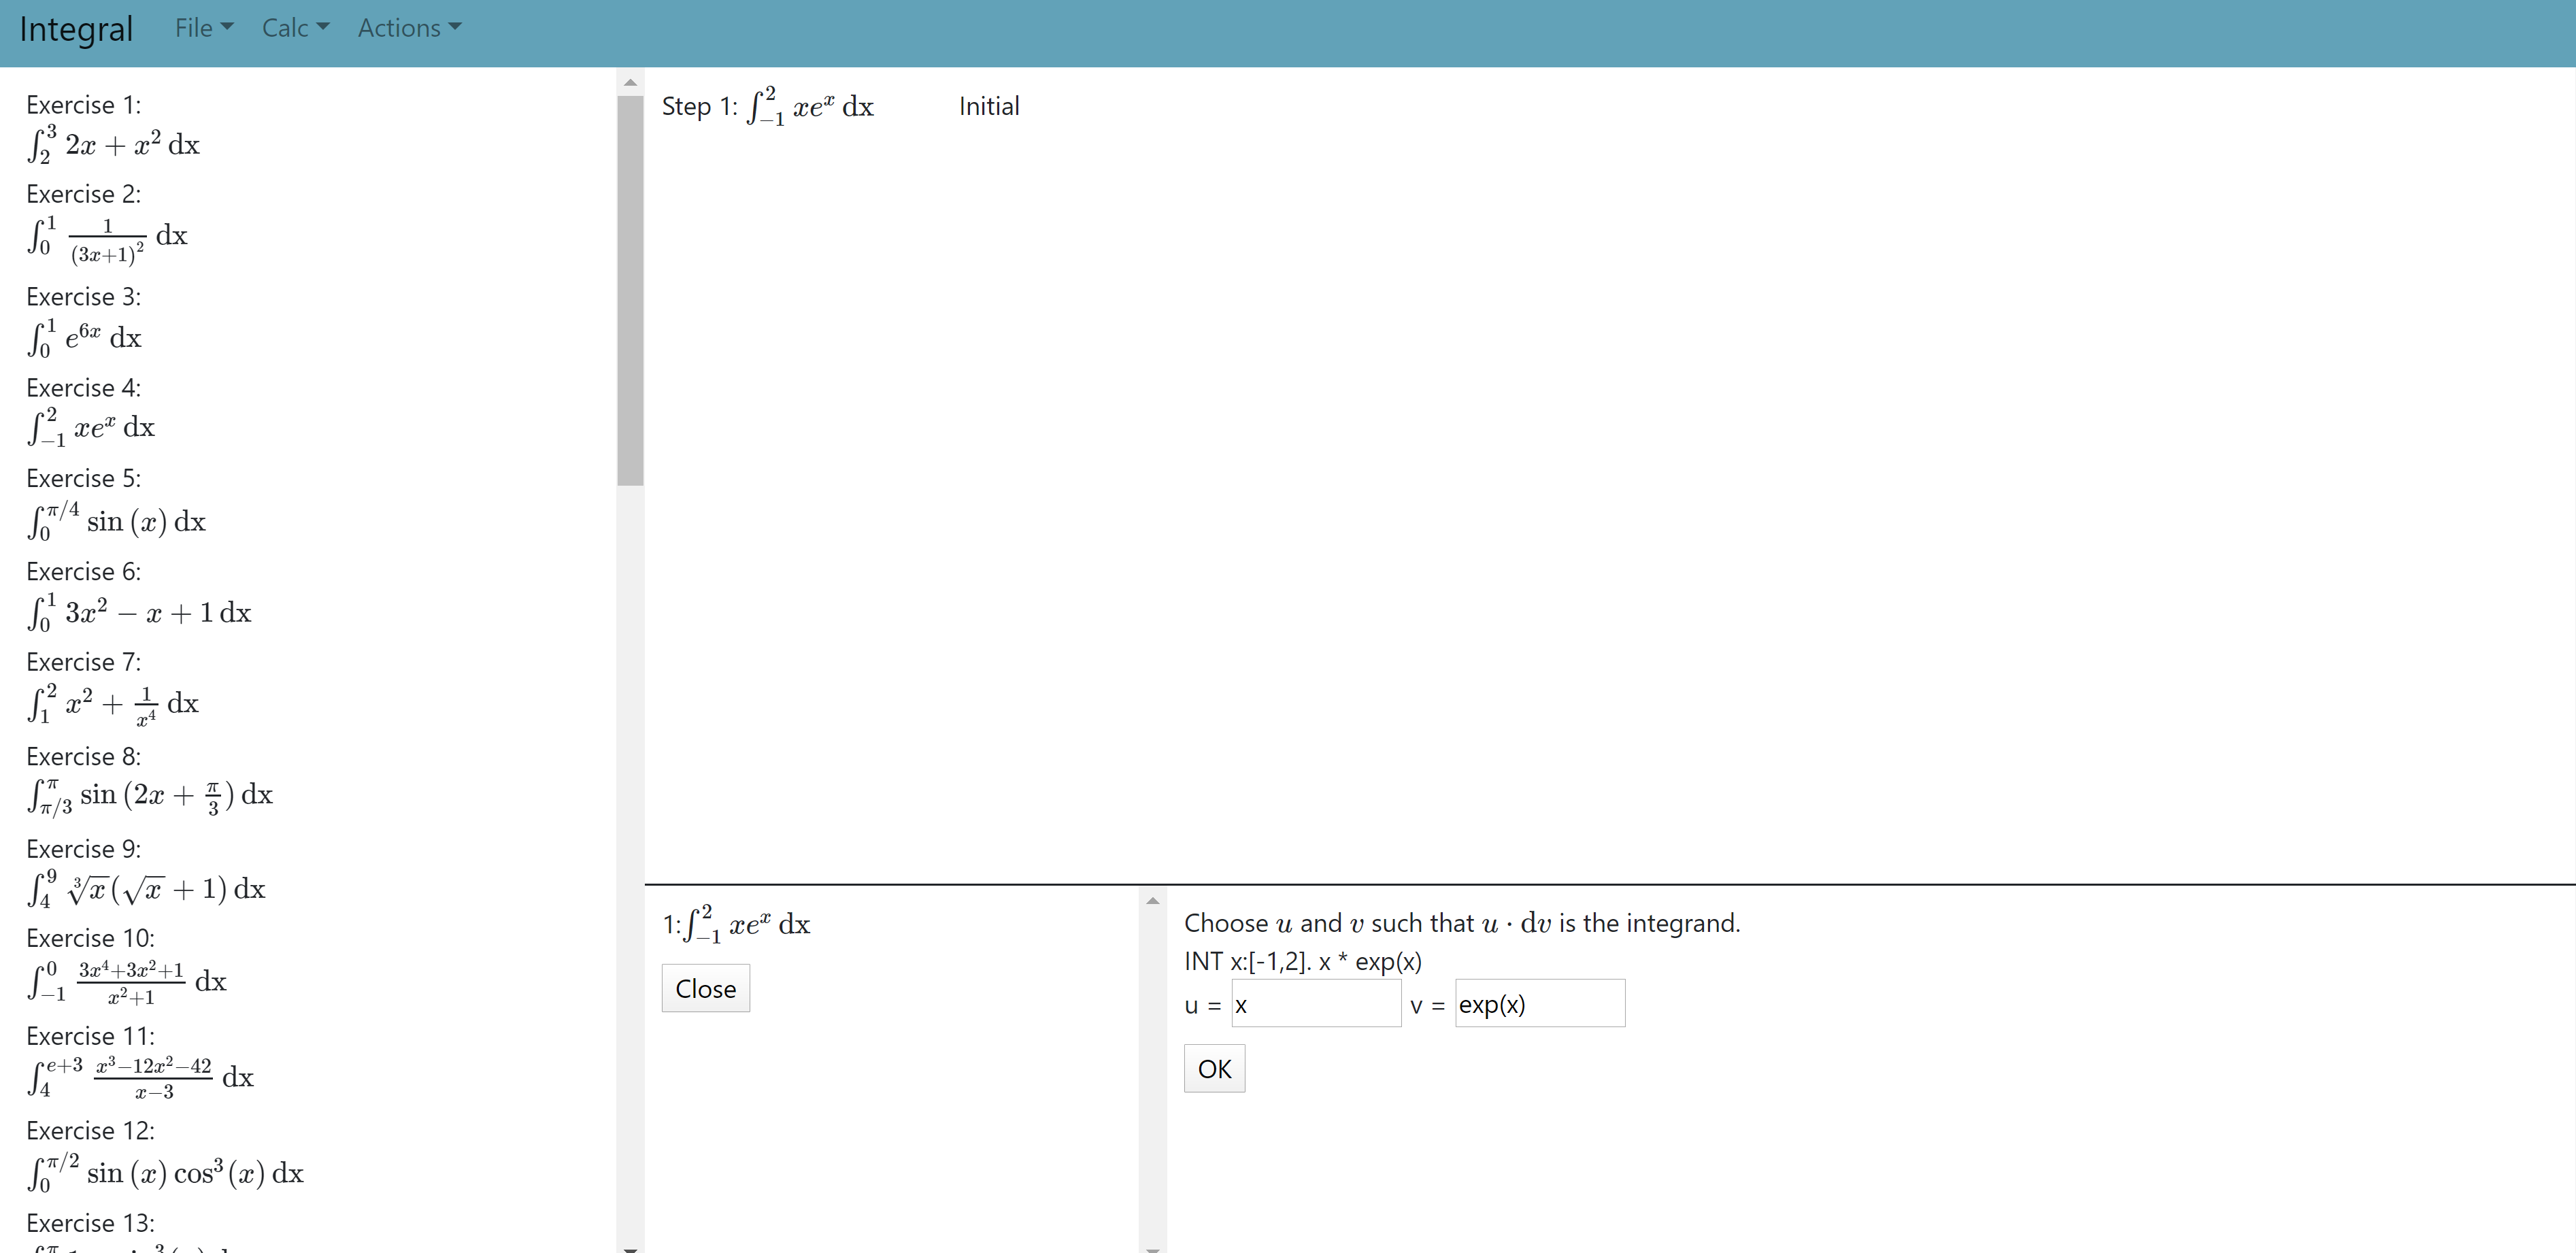
\includegraphics[width=13cm, height=7cm]{14.png}\\
The paradiam of integrate by parts rule is rewriting $u(x)v'(x)dx$ to $u(x)dv(x)$, the first text area represents u(x), and the second represents v(x). Note that if the user's input u(x) and v(x) cannot promise that $u(x)dv(x)\,==\,u(x)d(x)dx$, \rom{5} will display an error message. In this example, we input $x$ and $e^{x}$. And get the result in \rom{3}:\\\\
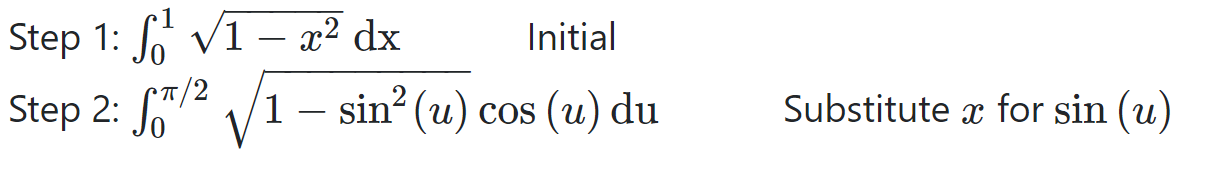
\includegraphics{30.png}\\
\subsubsection{Rewrite fraction}
Sometimes you may want to perform a partial fraction decomposition upon the integration body. For example, tongji7 exercise 10:
\begin{center}
$\int_{-1}^{0} \frac{3*x^4 + 3*x^2 + 1}{x^2 + 1} dx$
\end{center}
You can click the \colorbox{mygray}{Rewrite fraction} button to apply this rule.\\
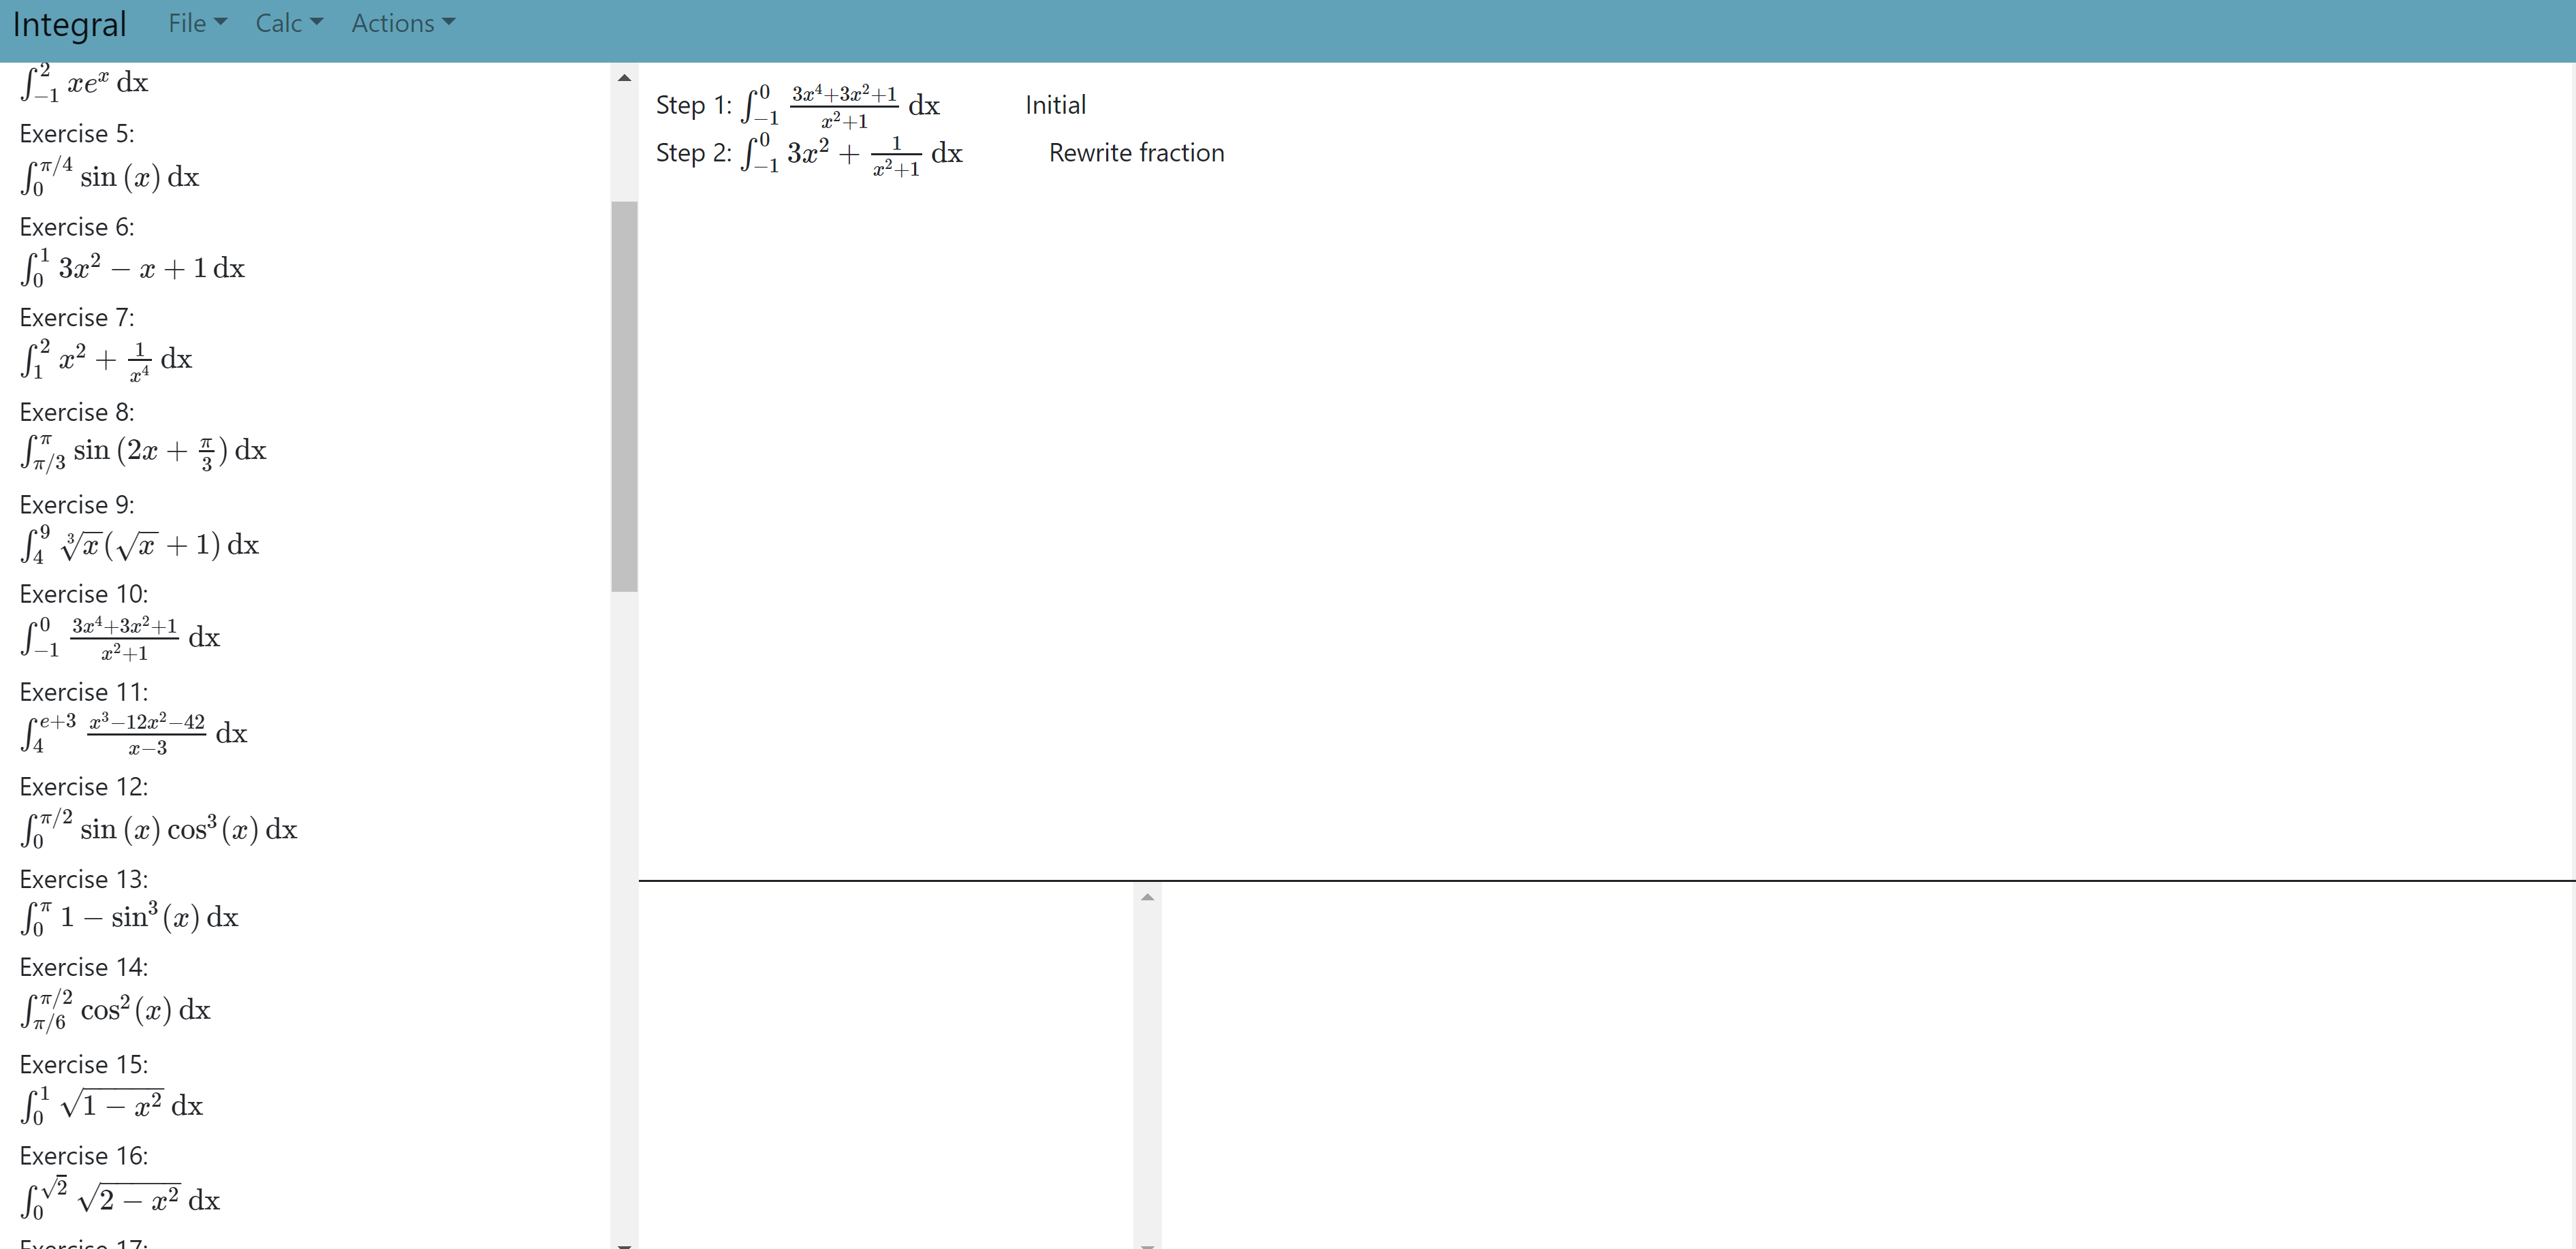
\includegraphics[width=13cm, height=7cm]{16.png}
\subsubsection{Rewrite}
Sometimes you may want to rewrite an expression to and equivalent form instead of a normal form to apply other rules. For example, tongji7 exercise 26:
\begin{center}
$\int_{-\pi/2}^{\pi/2} \sqrt{cos(x) - cos^{3}x} dx$
\end{center}
We can observe that if we rewrite the term $cos(x) - cos^{3}(x)$ to $cos(x)(1 - cos^{2}(x))$, then we can use trigonometric identities to rewrite $1-cos^{2}(x)$ to $sin(x)$. In order to do this, we need guarantee two thing, first, user can select arbitrary terms in the integral body as long as it is a valid expression, second, the expression which user writes is equivalent to the selected ones. Click \colorbox{mygray}{Equation substitution} button and choose the integral in \rom{4}. Then the \rom{5} becomes:\\
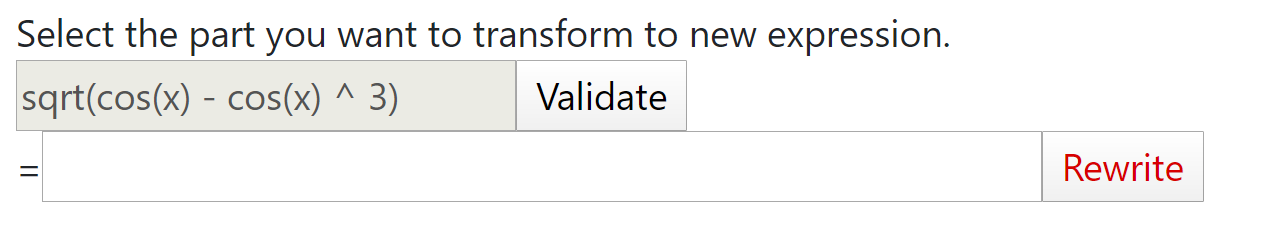
\includegraphics{17.png}\\
The first text area has been filled with the selected integral body, we need to use mouse to select the sub-expression which want to rewrite, like this:\\
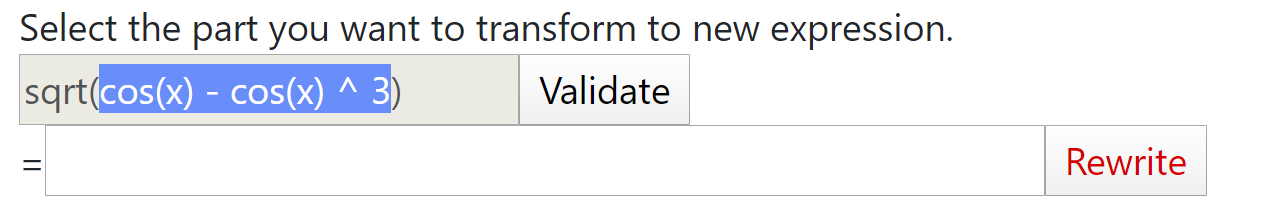
\includegraphics{18.png}\\
After select $cos(x) - cos^{3}(x)$, click the \colorbox{mygray}{Validate} to determine the user whether selects a valid expression, if not, \rom{5} will display error message. If it is valid, the third line left-hand part will show the selected expression:\\
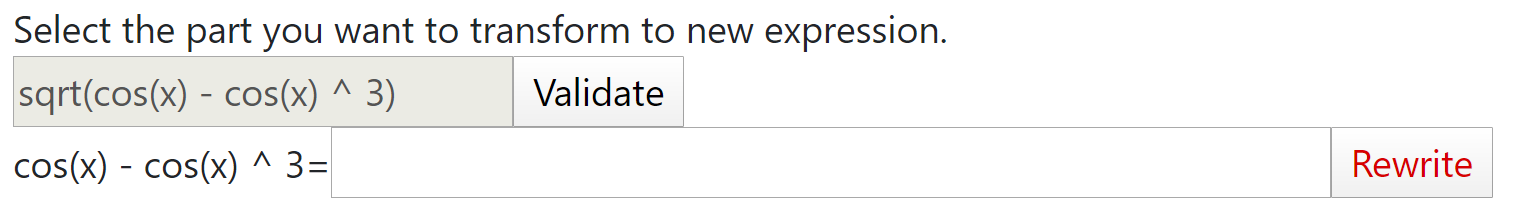
\includegraphics{19.png}\\
Then you can write the equivalent experssion in the second area and click \colorbox{mygray}{Rewrite} to rewrite the expression. Note that HolPy will also check the rewrite expression is whether equivalent to the initial expression. \\
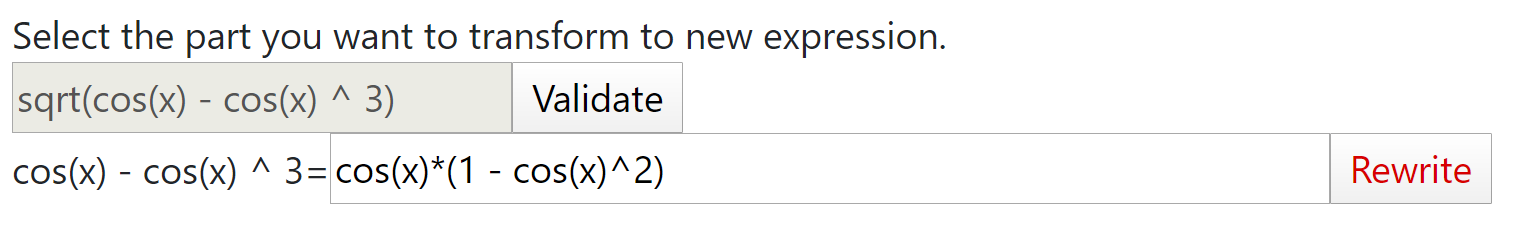
\includegraphics{20.png}\\
If all these staffs have done with no error, the rewrite operation is successful and \rom{3} becomes:\\\\
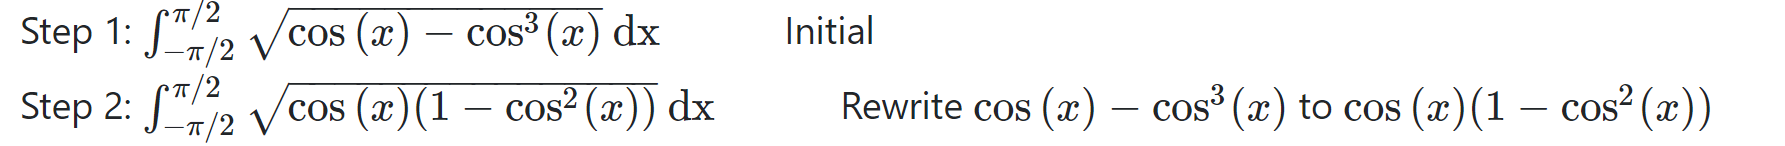
\includegraphics[width=14.5cm]{21.png}\\
\subsubsection{Trigonometric identities}
Application of trigonometric identities is common in solving integrals. For example, the tongji7 exercise 14:
\begin{center}
$\int_{\pi/6}^{\pi/2} cos^{2}(x) dx$
\end{center}
On solution is to reduce the power of cos by increasing the angle. To do this, click \colorbox{mygray}{Trig identity}, and select the integral in \rom{4}.Then the \rom{5} becomes:\\
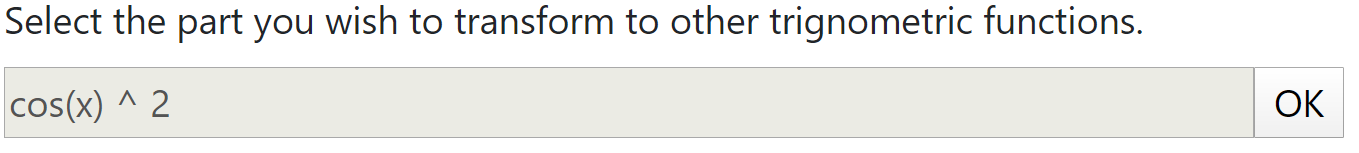
\includegraphics{22.png}\\
Like 3.4.6, user need to select the trigonometric function part which need to be transformed, in this example, select $cos^{2}(x)$:\\\\
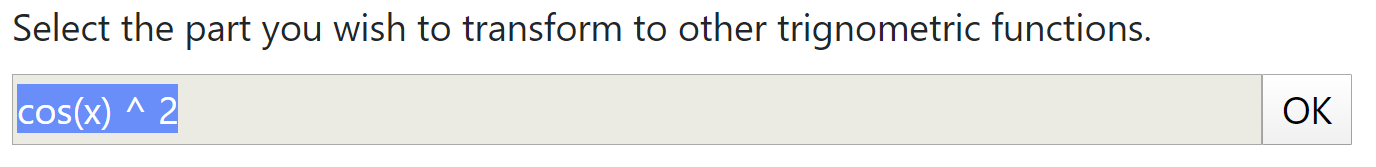
\includegraphics{23.png}\\
Click the \colorbox{mygray}{OK} button, the \rom{5} will displays all the possible transformations upon the selected one:\\\\
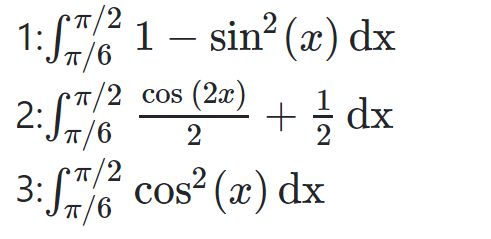
\includegraphics{24.png}\\
User need to click the transformation which they prefer and the rule is finished, \rom{3} occurs a new step:\\\\
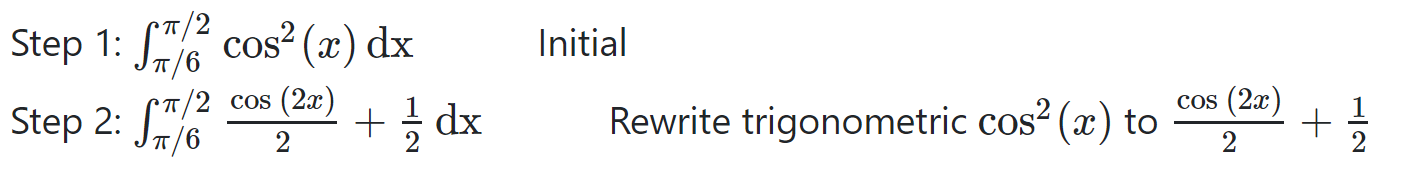
\includegraphics[width=13cm]{32.png}\\
\subsubsection{Split an integral}
Sometimes when users deal with the integral whose body has abstract values or user may want to do a substitution with a function which is non-monotonic function in the integral region. User need to split the integral region into several parts. Like tongji7 exercise 36:
\begin{center}
$\int_{1/e}^{e} \left| \log{(x)} \right| dx$
\end{center}
We know that when $x\,<\,1$, $log(x)\,<\,0$, so in $(1/e,\,1)$, $\left| \log{(x)} \right|\,=\,-\log{(x)}$. In order to eliminate the abstract value, we need to tell HolPy the point to split the region. Click \colorbox{mygray}{Split region} button and select the integral in \rom{4}, the \rom{5} becomes:\\\\

\includegraphics{25.png}\\
User need to fill the text area with the point to split on and click \colorbox{mygray}{OK} to finish this rule application, if the point is not in the range of integral region, there will be an error message. HolPy will spilt on the point and make the selected integral to a sum of two integrals. The \rom{3} becomes:\\
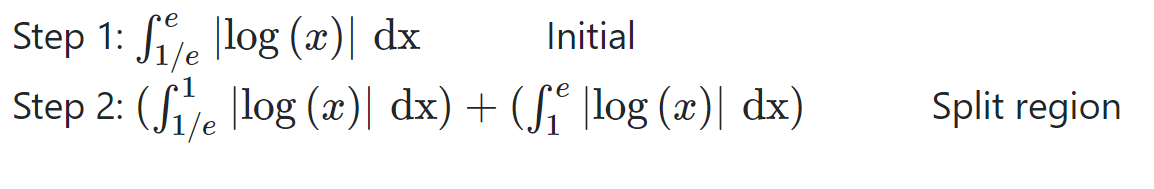
\includegraphics[width=14.5cm]{26.png}\\
\subsubsection{Solve equations}
If we encounter an integral which unfortunately cannot be solved by the all the previous rules, maybe we could try the Solving equations rules. This rule For instance, if an integral I can be written
in the form $X\,−\,cI$, where $X$ is any expression (containing no or simpler integrals),
and $c$ is a constant not equal to $−1$, then we can solve the equation $I\, =\, X\, −\, cI$
to obtain $I\, =\, X/(c\, +\, 1)$. Tongji7 Interesting 1 is an example of this form:
\begin{center}
$\int_{0}^{pi/2} \frac{\sqrt{sin(x)}}{\sqrt{sin(x)} + \sqrt{cos(x)}} dx$
\end{center}
By applying several of the previous rules, \rom{3} becomes:\\
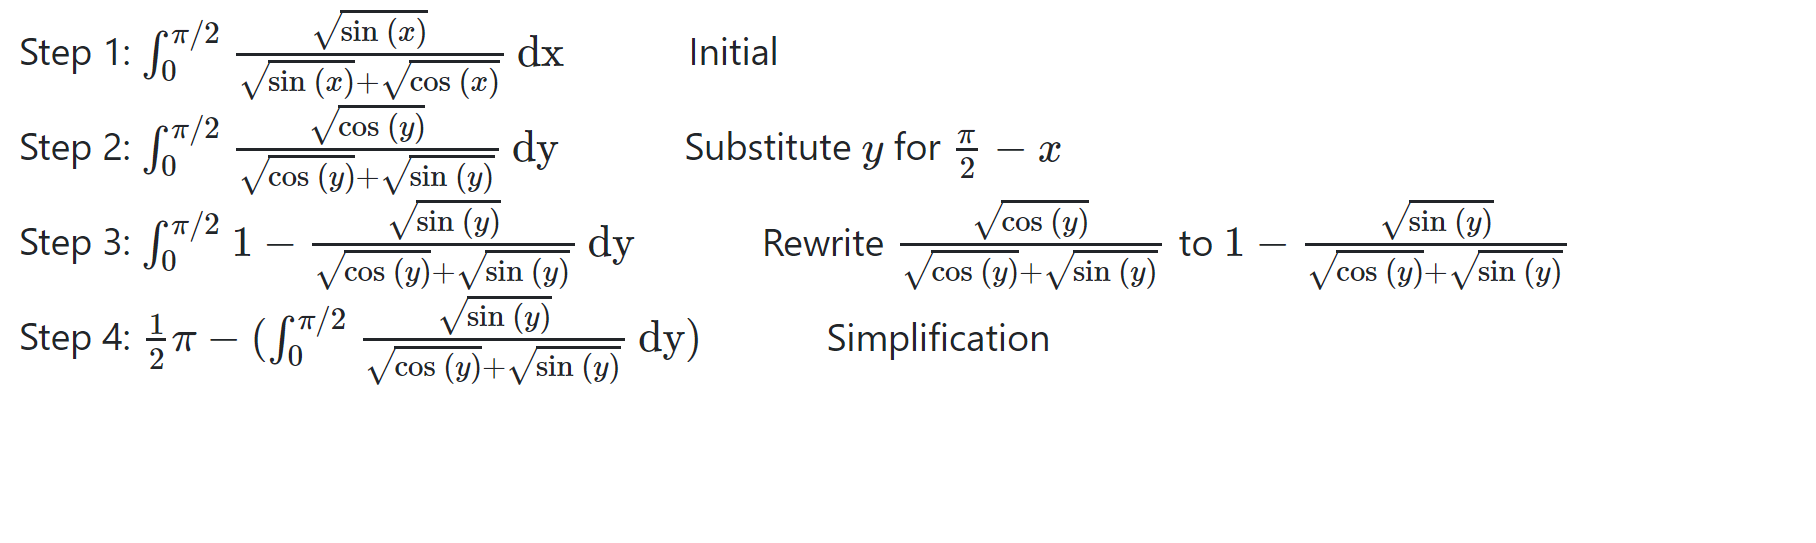
\includegraphics[width=14.5cm, height=6cm]{27.png}
We can observe that if we let I be the equal to original integral in step 1, step4 becomes $\frac{\pi}{2}\,-\,I$, and step1 = step4, then we get the answer $\frac{pi}{4}$. Click the \colorbox{mygray}{Integrate by equation} button, \rom{5} becomes:\\
\\
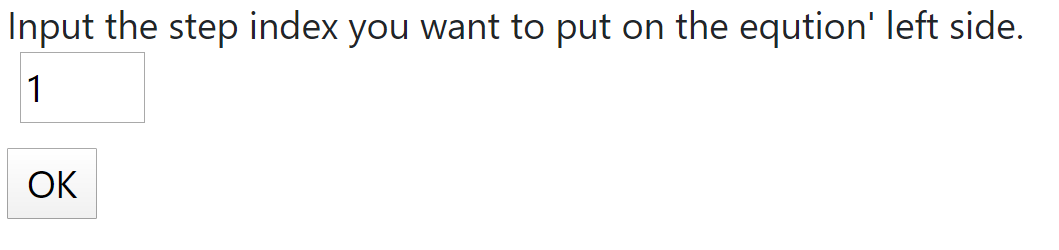
\includegraphics{28.png}\\
User need to input the step index to make equation with current step, this example we will fill with $1$. Then click \colorbox{mygray}{OK}. Then we get the answer $\frac{\pi}{4}$\\
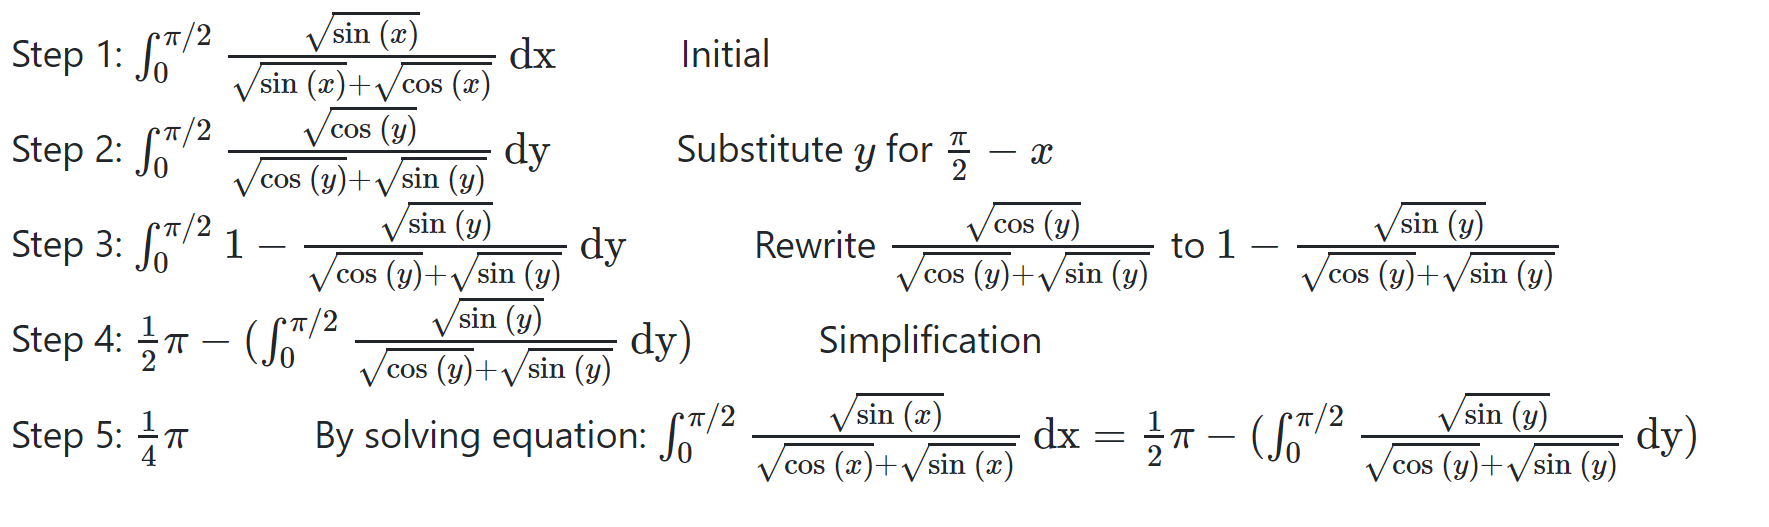
\includegraphics[width=14.5cm, height=6cm]{29.png}


\end{document}